\chapter{Analisys and result discussion}
In the previous section the author has explained the steps followed to forecast electricity prices and explore the different predictors' influence. We are now discussing the configuration fixed for the hourly, daily, monthly and yearly setups, and the results obtained on each case.

The length of the time series to be used, the forecasting horizon, the number of lags and the predictors to be included have to be selected for each specific scenario. They have been chosen with the help of a topic expert, concretely my Thesis' Supervisor.

For the hourly and daily levels, the pre-pandemic and post-war markets are being studied.

\newpage
\section{Hourly analysis}
In this case the author is working with a 6 months data window. It has been decided to make 168 hours ahead forecasts (1 week). The lags in use try to model the autocorrelation, and are the following: 1, 2, 12, 23, 24, 36, 71, 72, 167 and 168. Apart, other predictors are included to add extra information to the model:

\begin{itemize}
    \item \textbf{Date predictors:} Hour, day and day of week.
    \item \textbf{Demand:} The total energy demand.
    \item \textbf{Generation:} Wind, hydropower, nuclear, solar, combined cycle and coal generation technologies measurements.
\end{itemize}

Cross validation is applied using 15 windows, with step size of 191.

As the author mentioned, the energy market should have changed due to the Covid pandemic and specially to the war in Ukraine. These differences between current and past market will be analyzed.

\subsection{Pre-pandemic scenario}
The data used for the pre-pandemic scenario experiments goes from 2018-10-01 to 2019-03-31, before the increase in energy prices shown in Figure \ref{fig:spot-price-series-month}. In Table \ref{tab:cv-hourly-prep} you can find the performance of different models for the cross validation phase. The best one is a Random Forest, it is the one the author will use to make the final forecast.

\begin{table}[H]
\centering
\begin{tabular}{@{}l|l|l@{}}
\toprule
Model & MASE  & Modelling time (s)  \\ \midrule
RF    & 1.196 & 192.24              \\
GBT   & 1.264 & 113.17              \\
kNN   & 1.919 & 97.52               \\ \bottomrule
\end{tabular}
\caption{Model performance comparison trained over the hourly pre-pandemic energy price.}
\label{tab:cv-hourly-prep}
\end{table}

The final forecast is generated as explained in Chapter \ref{ch:methodology}, using the train split to build the model and the test to give a final estimation of the performance. The forecast is shown in Figure \ref{fig:forecast-hourly-pre}, obtaining a MASE of 1.18. As it can be seen, the model is correctly capturing data patterns and materialising these insights in the forecast.

\begin{figure}[H]
\centering
    \caption{Final forecasting of hourly pre-pandemic energy price.}
    \label{fig:forecast-hourly-pre}
    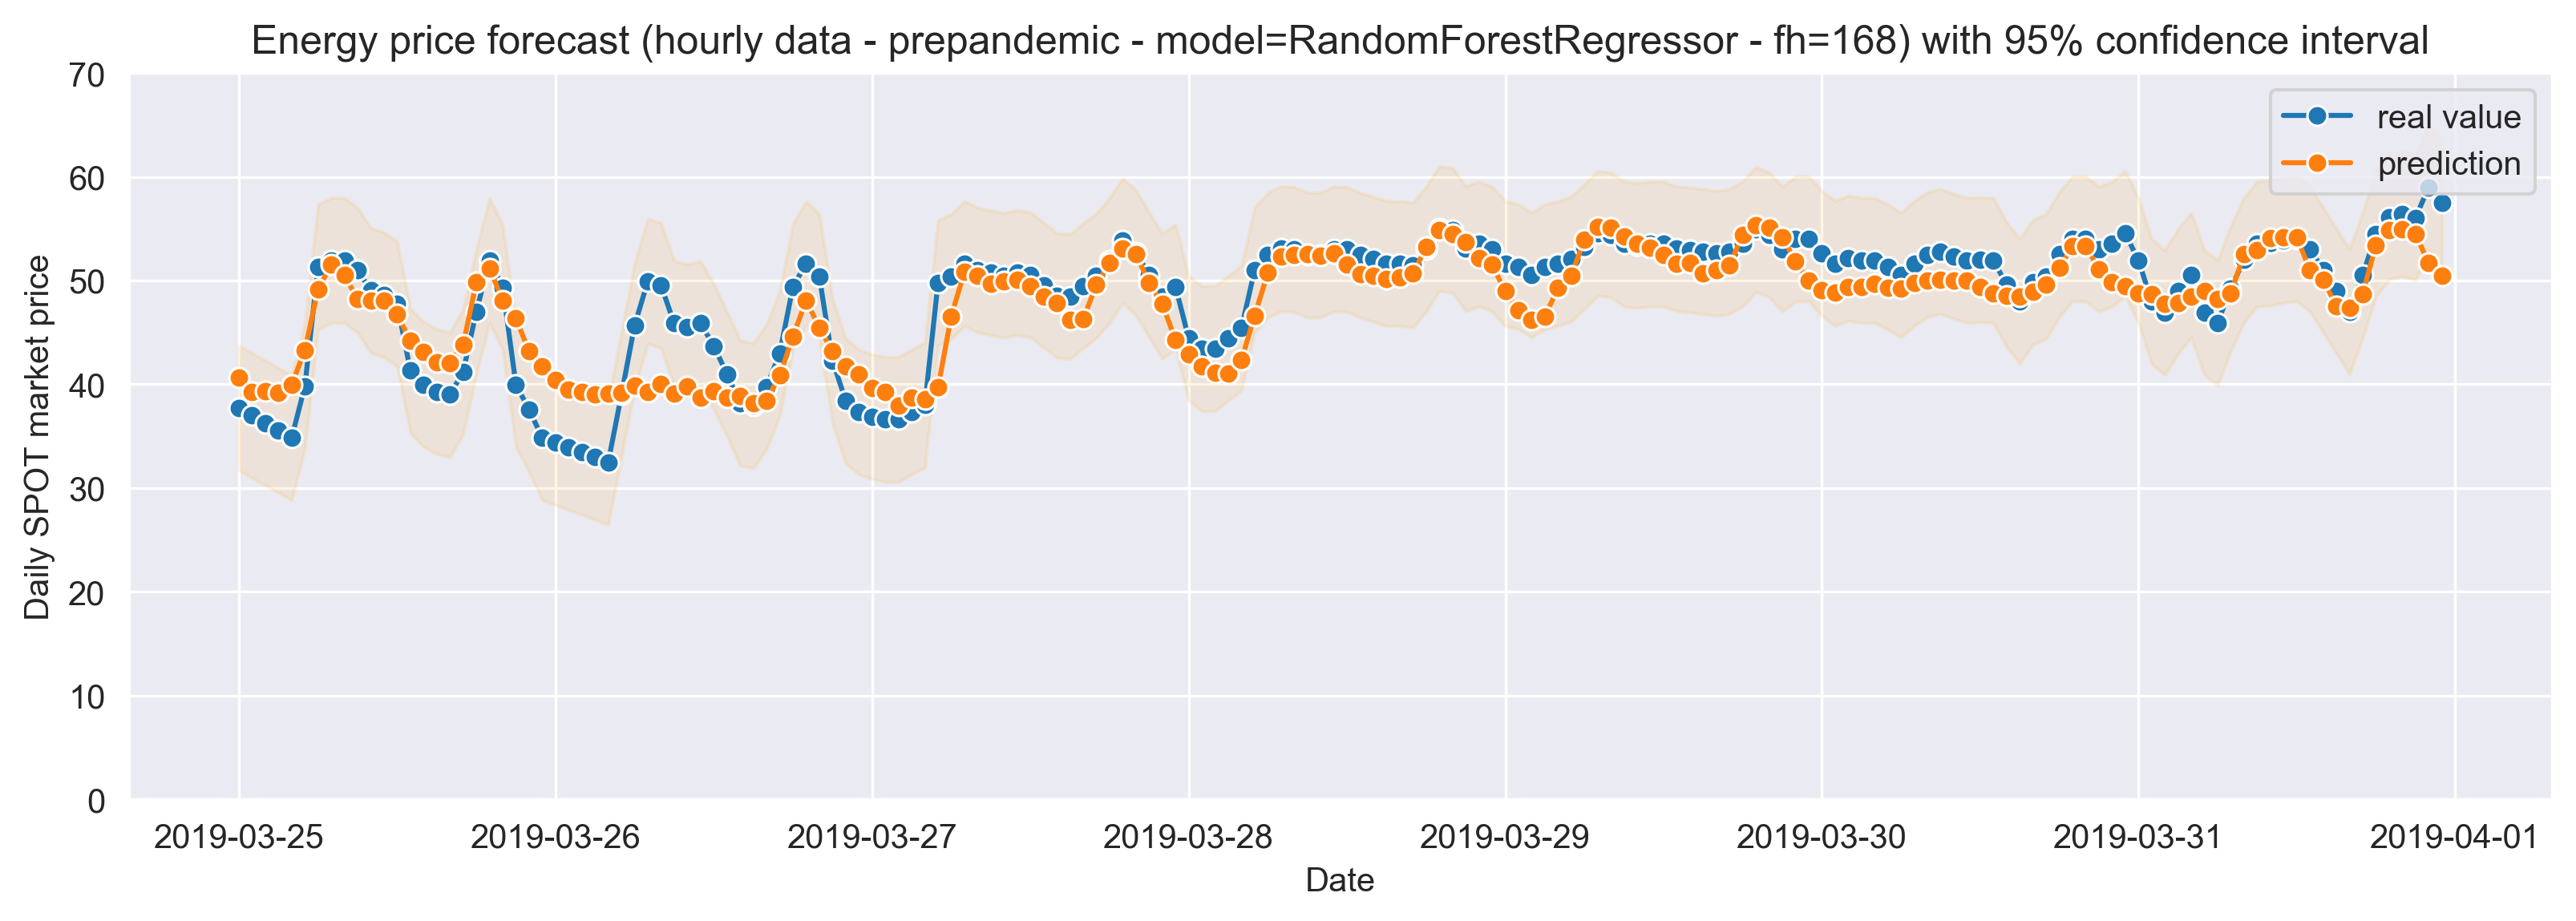
\includegraphics[scale=0.4]{images/analysis/forecast-hourly-pre}
\end{figure}

Which are the predictors that are specially influencing this forecast? Let's compute the SHAP values. In Figure \ref{fig:shap-hourly-pre} you can see them: a low SHAP value for a predictor observation means that that observation will decrease energy price, and vice-versa. The color assigned to each predictor observation depends on the value of that observation: blue means a low value, red means a high value.

So blue observations with low SHAP values mean that when that predictor takes a low value, the response lows its value too.

\begin{figure}[H]
\centering
    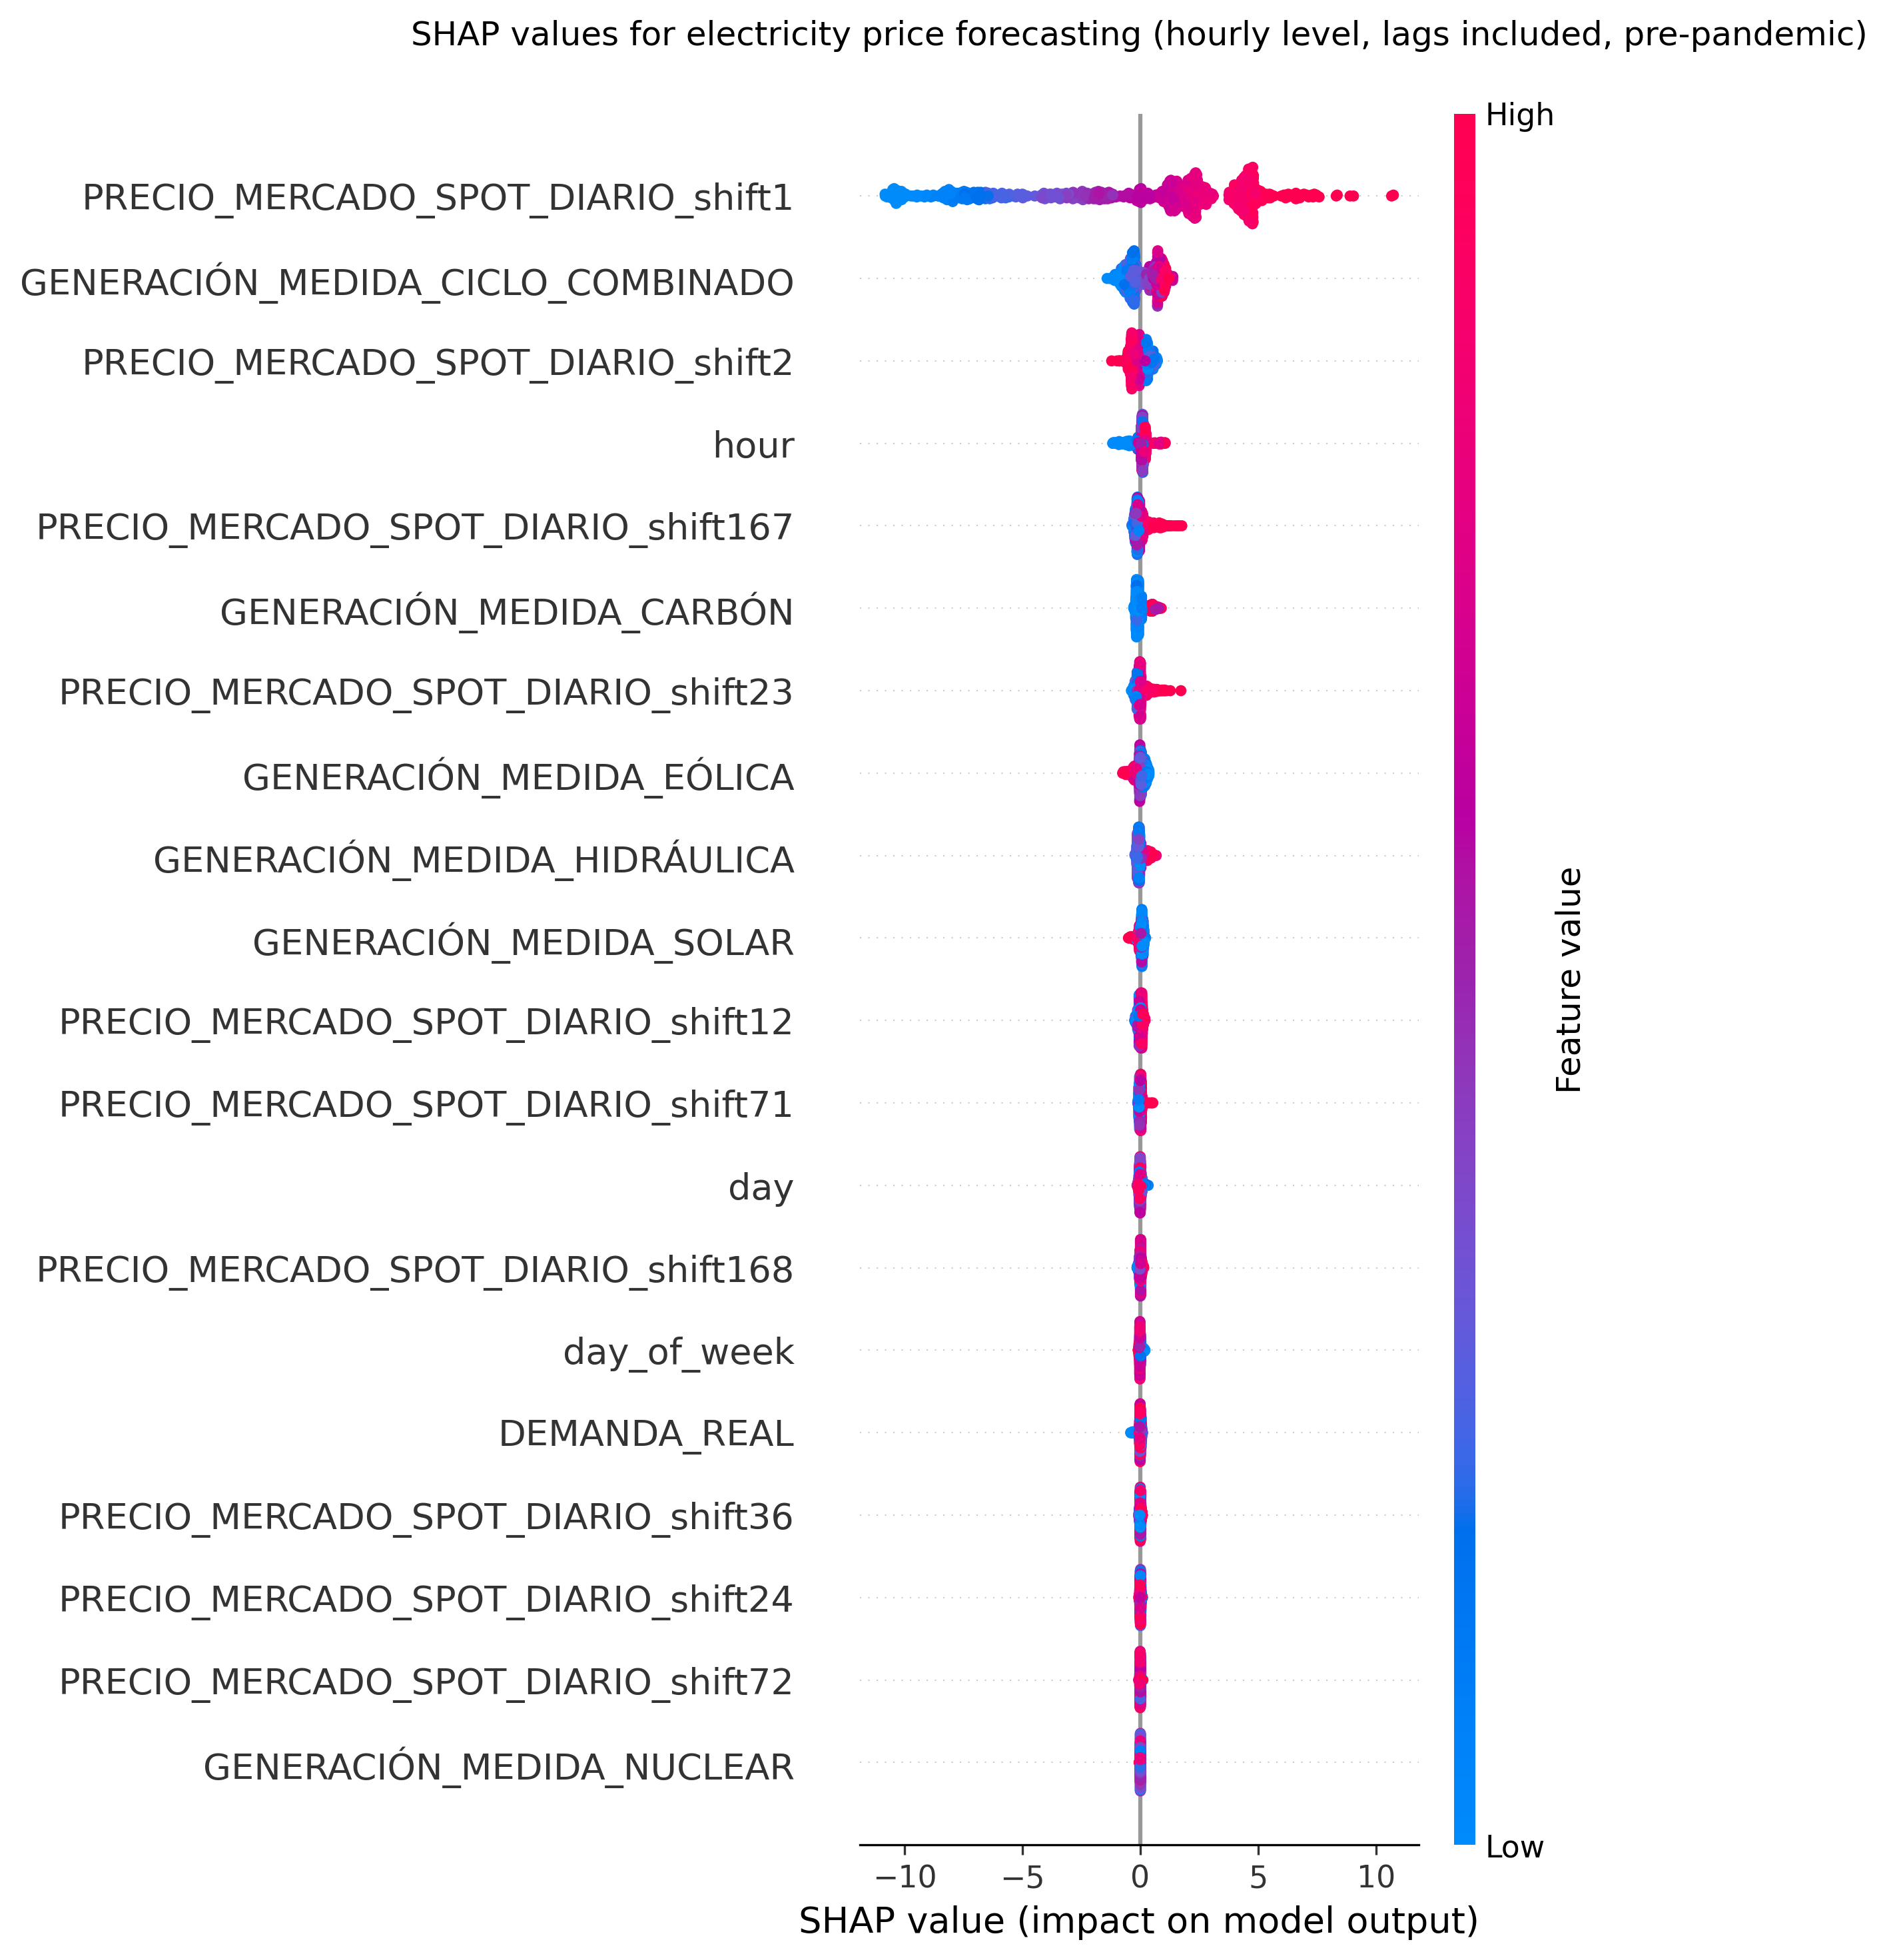
\includegraphics[width=0.7\linewidth]{images/analysis/shap-hourly-pre}
    \caption{SHAP values for the hourly pre-pandemic energy price forecasting.}
    \label{fig:shap-hourly-pre}
\end{figure}

See Figure \ref{fig:shap-hourly-pre}: the first lag has a lot of importance. Concretely, if the lag takes a low value (blue color), the response value will tend to be low too, and vice-versa. Lag two has also some importance, but in this case a low value in the lag means a higher value in the response and vice-versa. The third lag with more importance is 167, specially in the positive side, when it takes a high value the output does the same.

About the rest of predictors, combined cycle generation and hour seem to have some importance. If the generation by combined cycle is high, the price goes up and vice-versa. The price in earlier hours is usually cheaper than in the end of the day: this makes sense, being correlated with the demand which is lower during the night.


\subsection{Post-Ukraine war scenario}
The data in use goes from 2022-10-01 to 2023-03-31. In the model selection stage the author obtains the results described in Table \ref{tab:cv-hourly-post}.

% Please add the following required packages to your document preamble:
% \usepackage{booktabs}
\begin{table}[H]
\centering
\begin{tabular}{@{}l|l|l@{}}
\toprule
Model & MASE  & Modelling time (s)  \\ \midrule
RF    & 1,964 & 98.63               \\
GBT   & 2.081 & 67.17               \\
kNN   & 4.014 & 111.84              \\ \bottomrule
\end{tabular}
\caption{Model performance comparison trained over the hourly post-Ukraine war energy prices.}
\label{tab:cv-hourly-post}
\end{table}

The best-performing model, in this post-war scenario, is again the one based on Random Forests (RF). The final forecast is shown in Figure \ref{fig:forecast-hourly-post}: a final MAE of 1.702 has been obtained over the test partition. It can be checked how the model is correctly capturing the shape of the data.

\begin{figure}[H]
\centering
    \caption{Final forecasting of hourly post-war energy price.}
    \label{fig:forecast-hourly-post}
    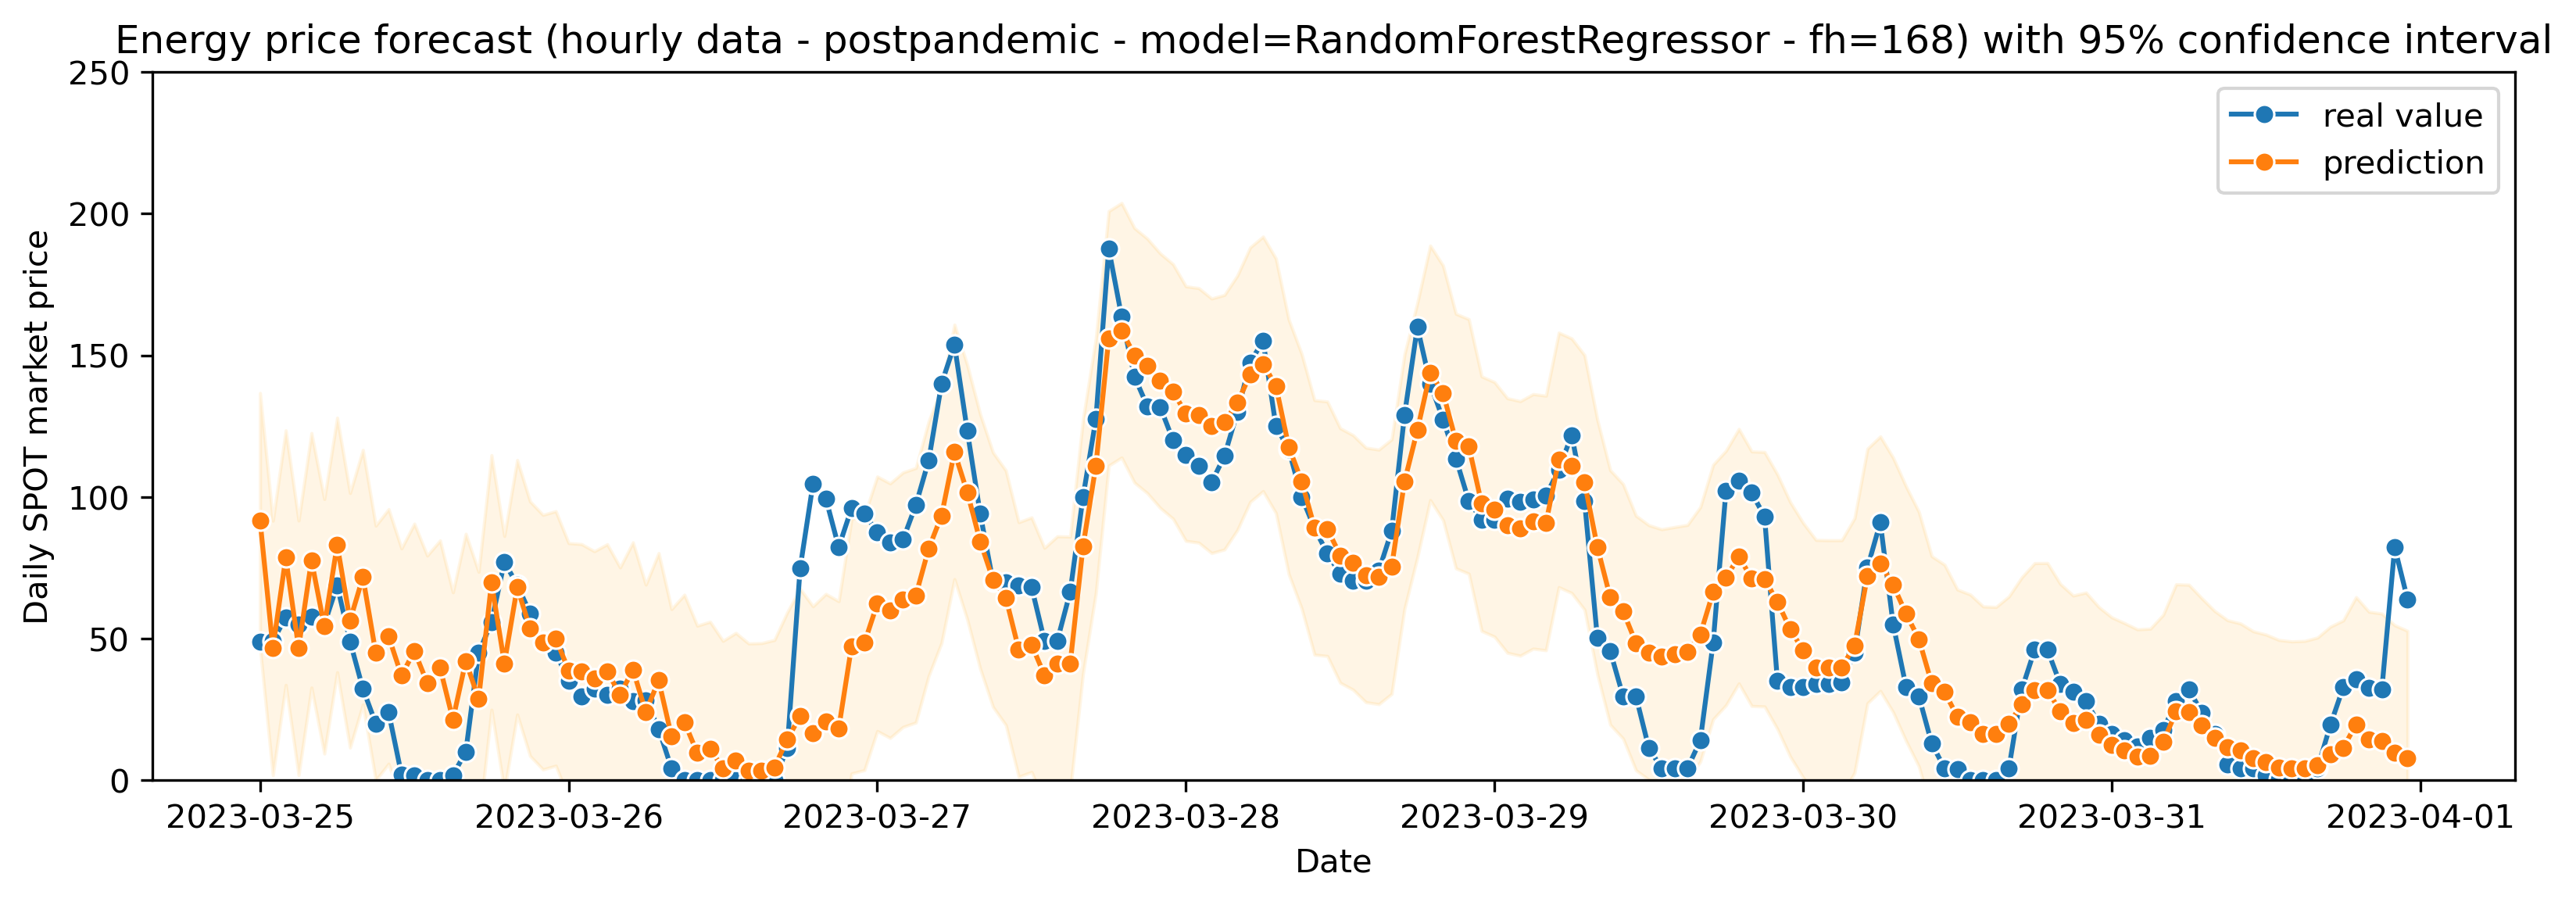
\includegraphics[scale=0.4]{images/analysis/forecast-hourly-post}
\end{figure}

In this case, the most important predictors are shown in Figure \ref{fig:shap-hourly-post}. Compared with the pre-pandemic series, we find similar predictors. A lag which seems more important than before is 23, but in general everything is similar.

\begin{figure}[H]
\centering
    \centering
    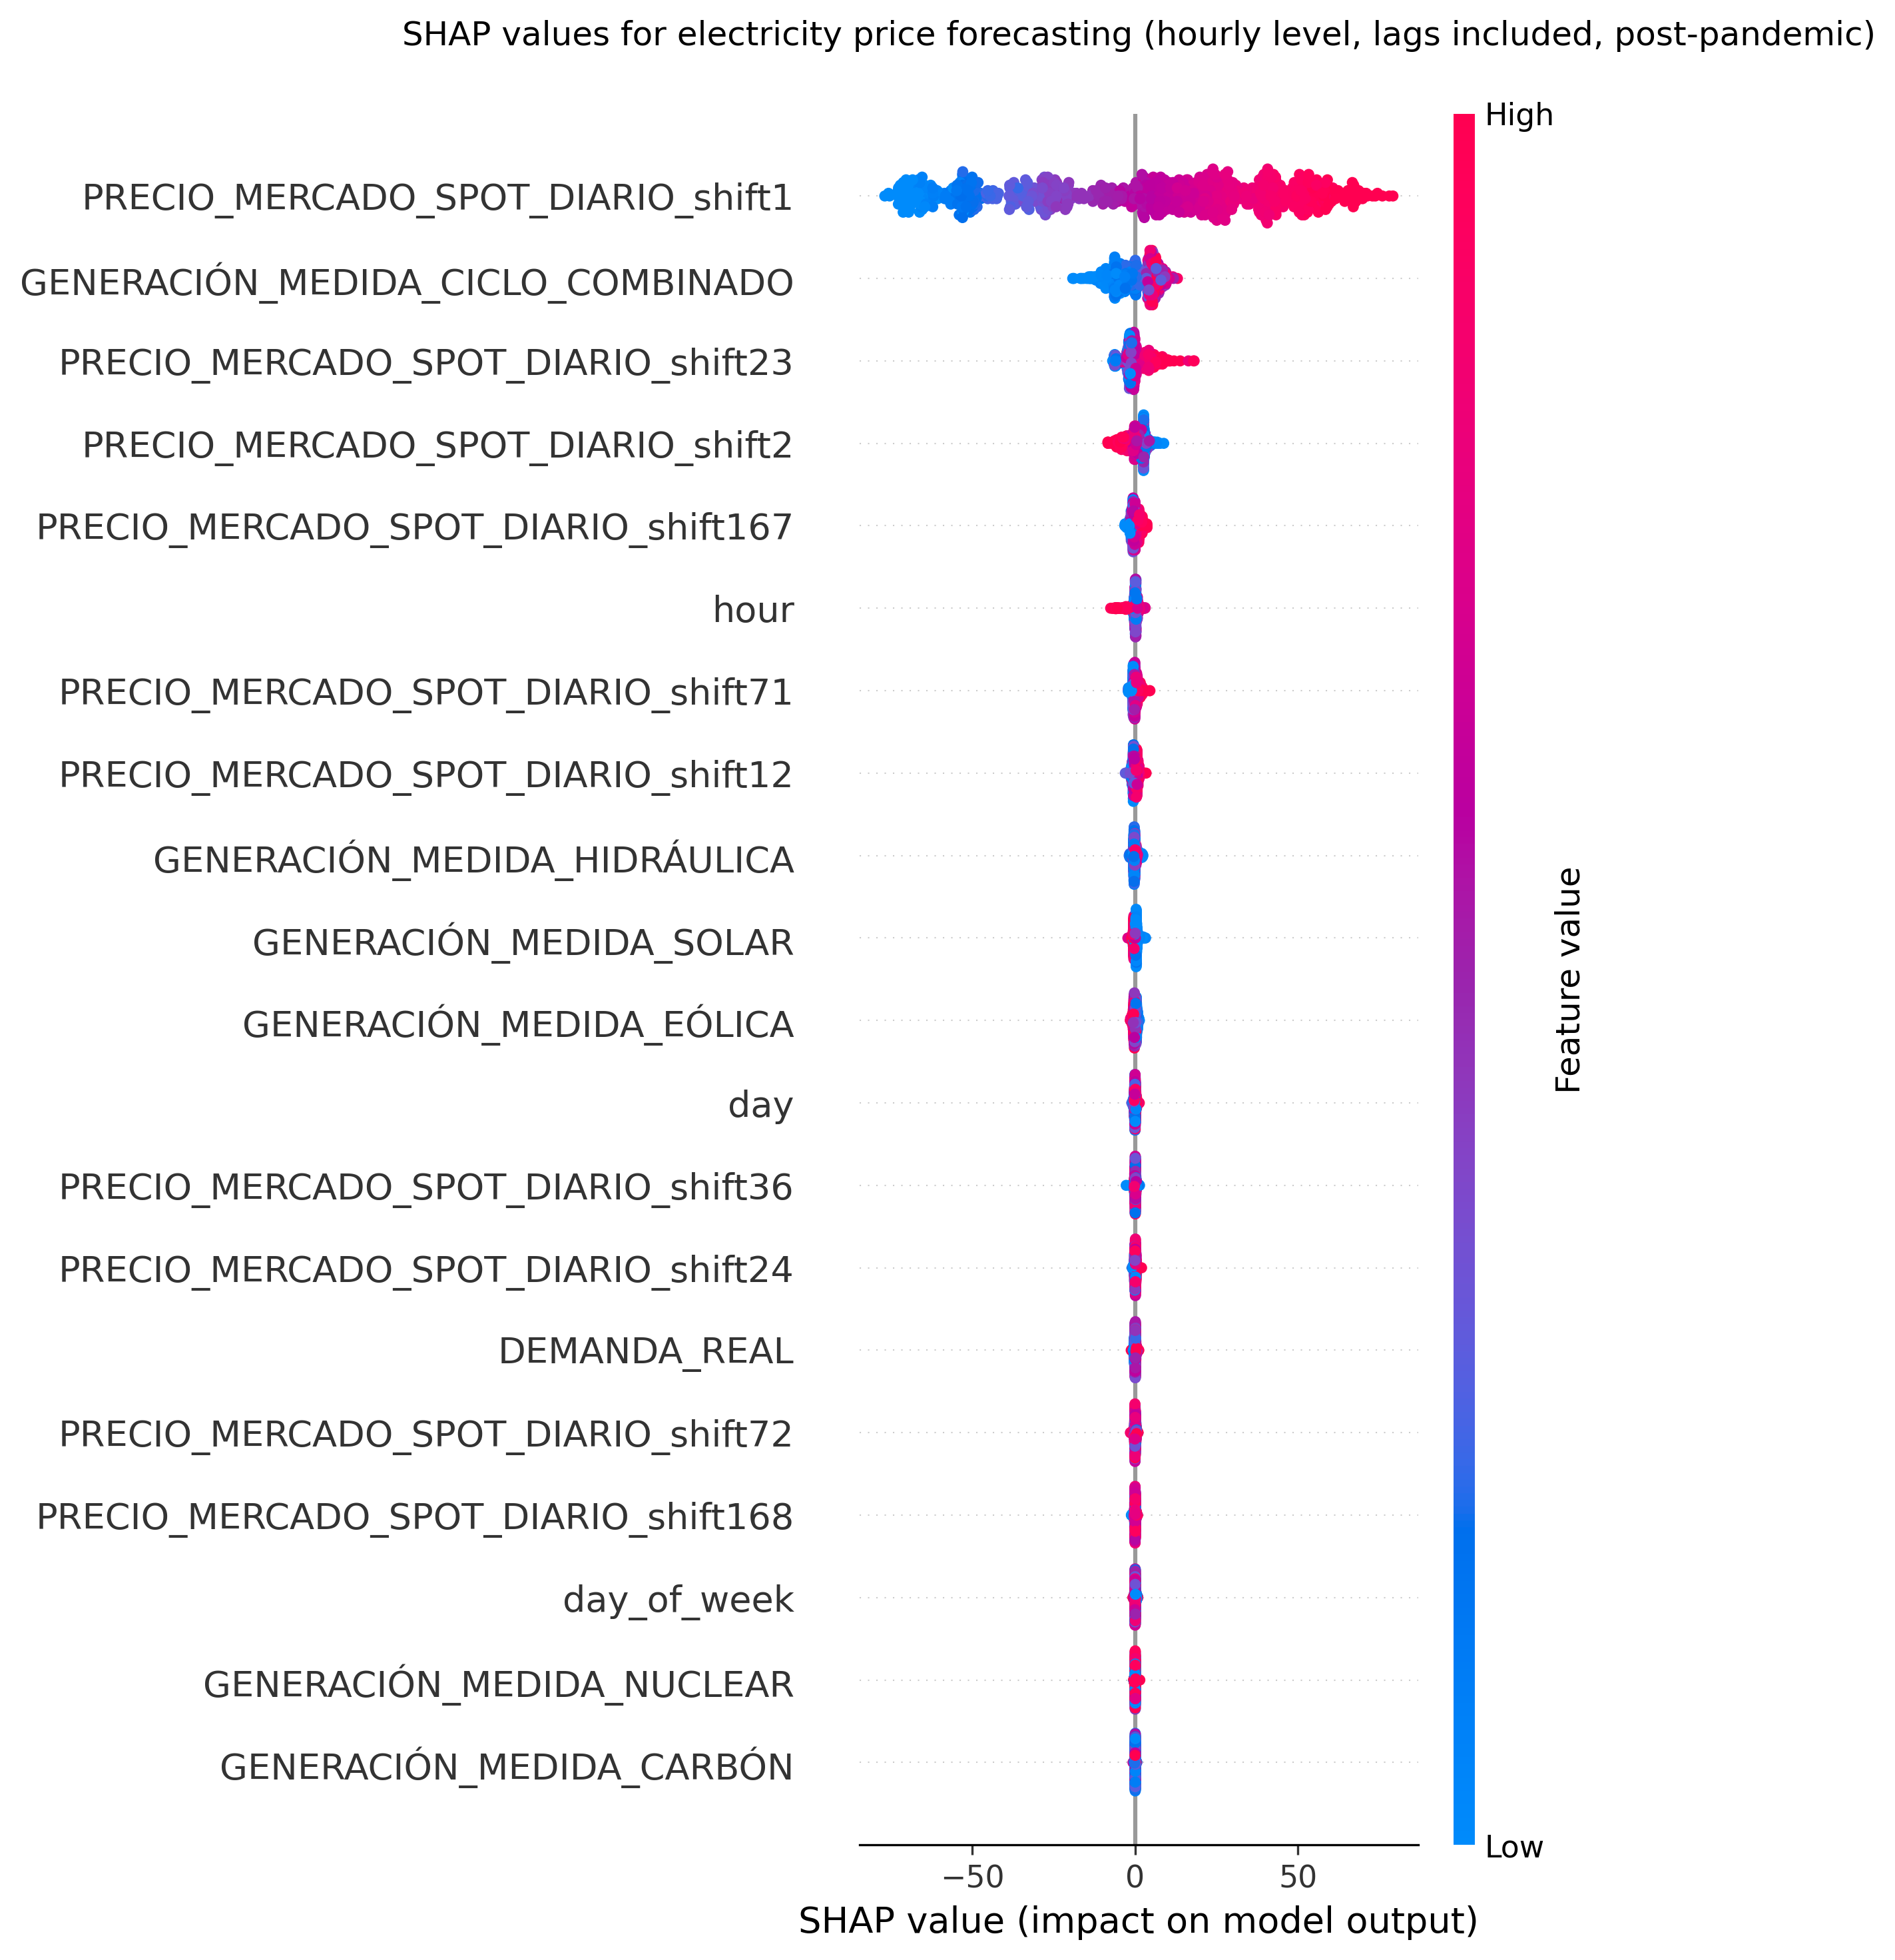
\includegraphics[width=0.7\linewidth]{images/analysis/shap-hourly-post}
    \caption{SHAP values for the hourly post-pandemic energy price forecasting.}
    \label{fig:shap-hourly-post}
\end{figure}

\subsection{Result discussion}
Both in the pre-pandemic and post-war scenarios the best performing models are Random Forests. Looking at the forecast graphs, they are correctly capturing the cyclicity present in data. Nevertheless, the forecast in the post-war case seems to have more uncertainty than the pre-pandemic one as the MASE obtained is higher and the confidence intervals are broader.

An important conclusion on this study is that combined cycle generation is a relevant predictor to model hourly prices. This makes sense, because as described in Chapter \ref{ch:electricity-market}, the commodity-based technologies normally set the energy price.

\newpage
\section{Daily analysis}
For the daily aggregation analysis 2 years of data are used, producing 30 days ahead forecasts. The lags added as predictors are 1, 2, 6, 7, 13, 14, 28, 30 and 31, apart we use the following new predictors:

\begin{itemize}
    \item \textbf{Date predictors:} Day, day of week, week of the year and month.
    \item \textbf{Gas price}
    \item \textbf{Coal price}
    \item \textbf{EU $CO_2$ allowances price}
\end{itemize}

\noindent Cross validation is applied again using 15 windows, but in this case the step size is 13.

\subsection{Pre-pandemic scenario}
The data used for the pre-pandemic scenario experiments ranges from 2018-04-01 to 2020-03-31. The model which performed the best was based on Gradient Boosting Trees (GBT), obtaining 1.394 as MASE, as can be seen in Table \ref{tab:cv-daily-prep}.

\begin{table}[H]
\centering
\begin{tabular}{@{}l|l|l@{}}
\toprule
Model & MASE  & Modelling time (s)  \\ \midrule
GBT   & 1.394 & 110.12 \\
RF    & 1.579 & 99.21  \\
kNN   & 1.965 & 156.20 \\ \bottomrule
\end{tabular}
\caption{Model performance comparison trained over the daily pre-pandemic energy price.}
\label{tab:cv-daily-prep}
\end{table}

The final forecast generated using GBT over holdout returns a MASE score of 1.043. The result can be visualized in Figure \ref{fig:forecast-daily-pre}: most of the true values remain inside the confidence interval generated during the forecast.

\begin{figure}[H]
\centering
    \caption{Final forecasting of daily pre-pandemic energy price.}
    \label{fig:forecast-daily-pre}
    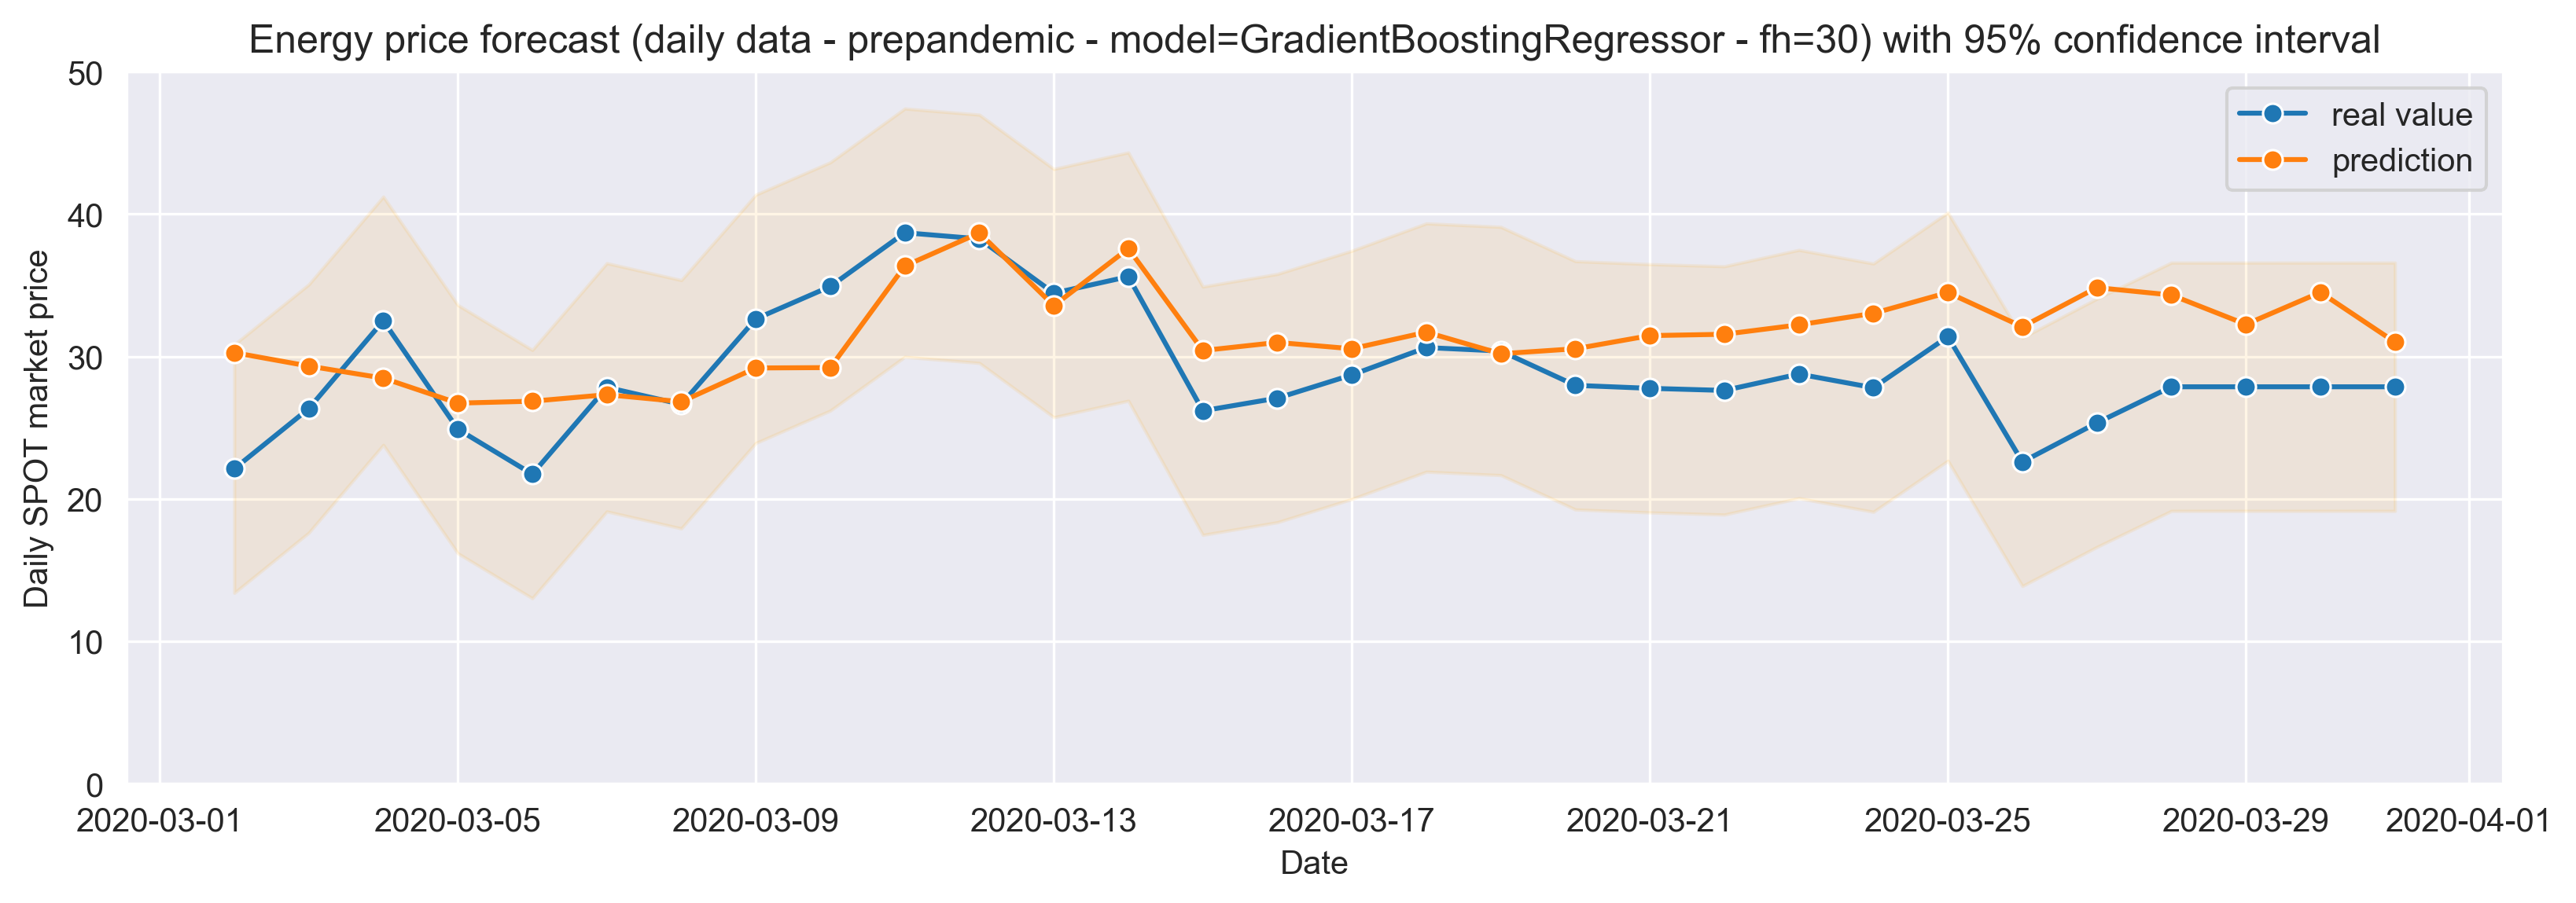
\includegraphics[scale=0.4]{images/analysis/forecast-daily-pre}
\end{figure}

Let's now compute the SHAP values for this model. In Figure \ref{fig:shap-daily-pre} we see how wind power, coal and combined cycle generation are the predictors influencing the forecast the most. As can be checked, high levels of wind power generation tend to lower the electricity price, while high levels of combined cycle or coal generation tend to increase it. Between the date predictors, the one which stands out the most is the week of the year. Finally, the most important lag is 1, something that makes sense as is the closest to the response.

\begin{figure}[H]
\centering
    \centering
    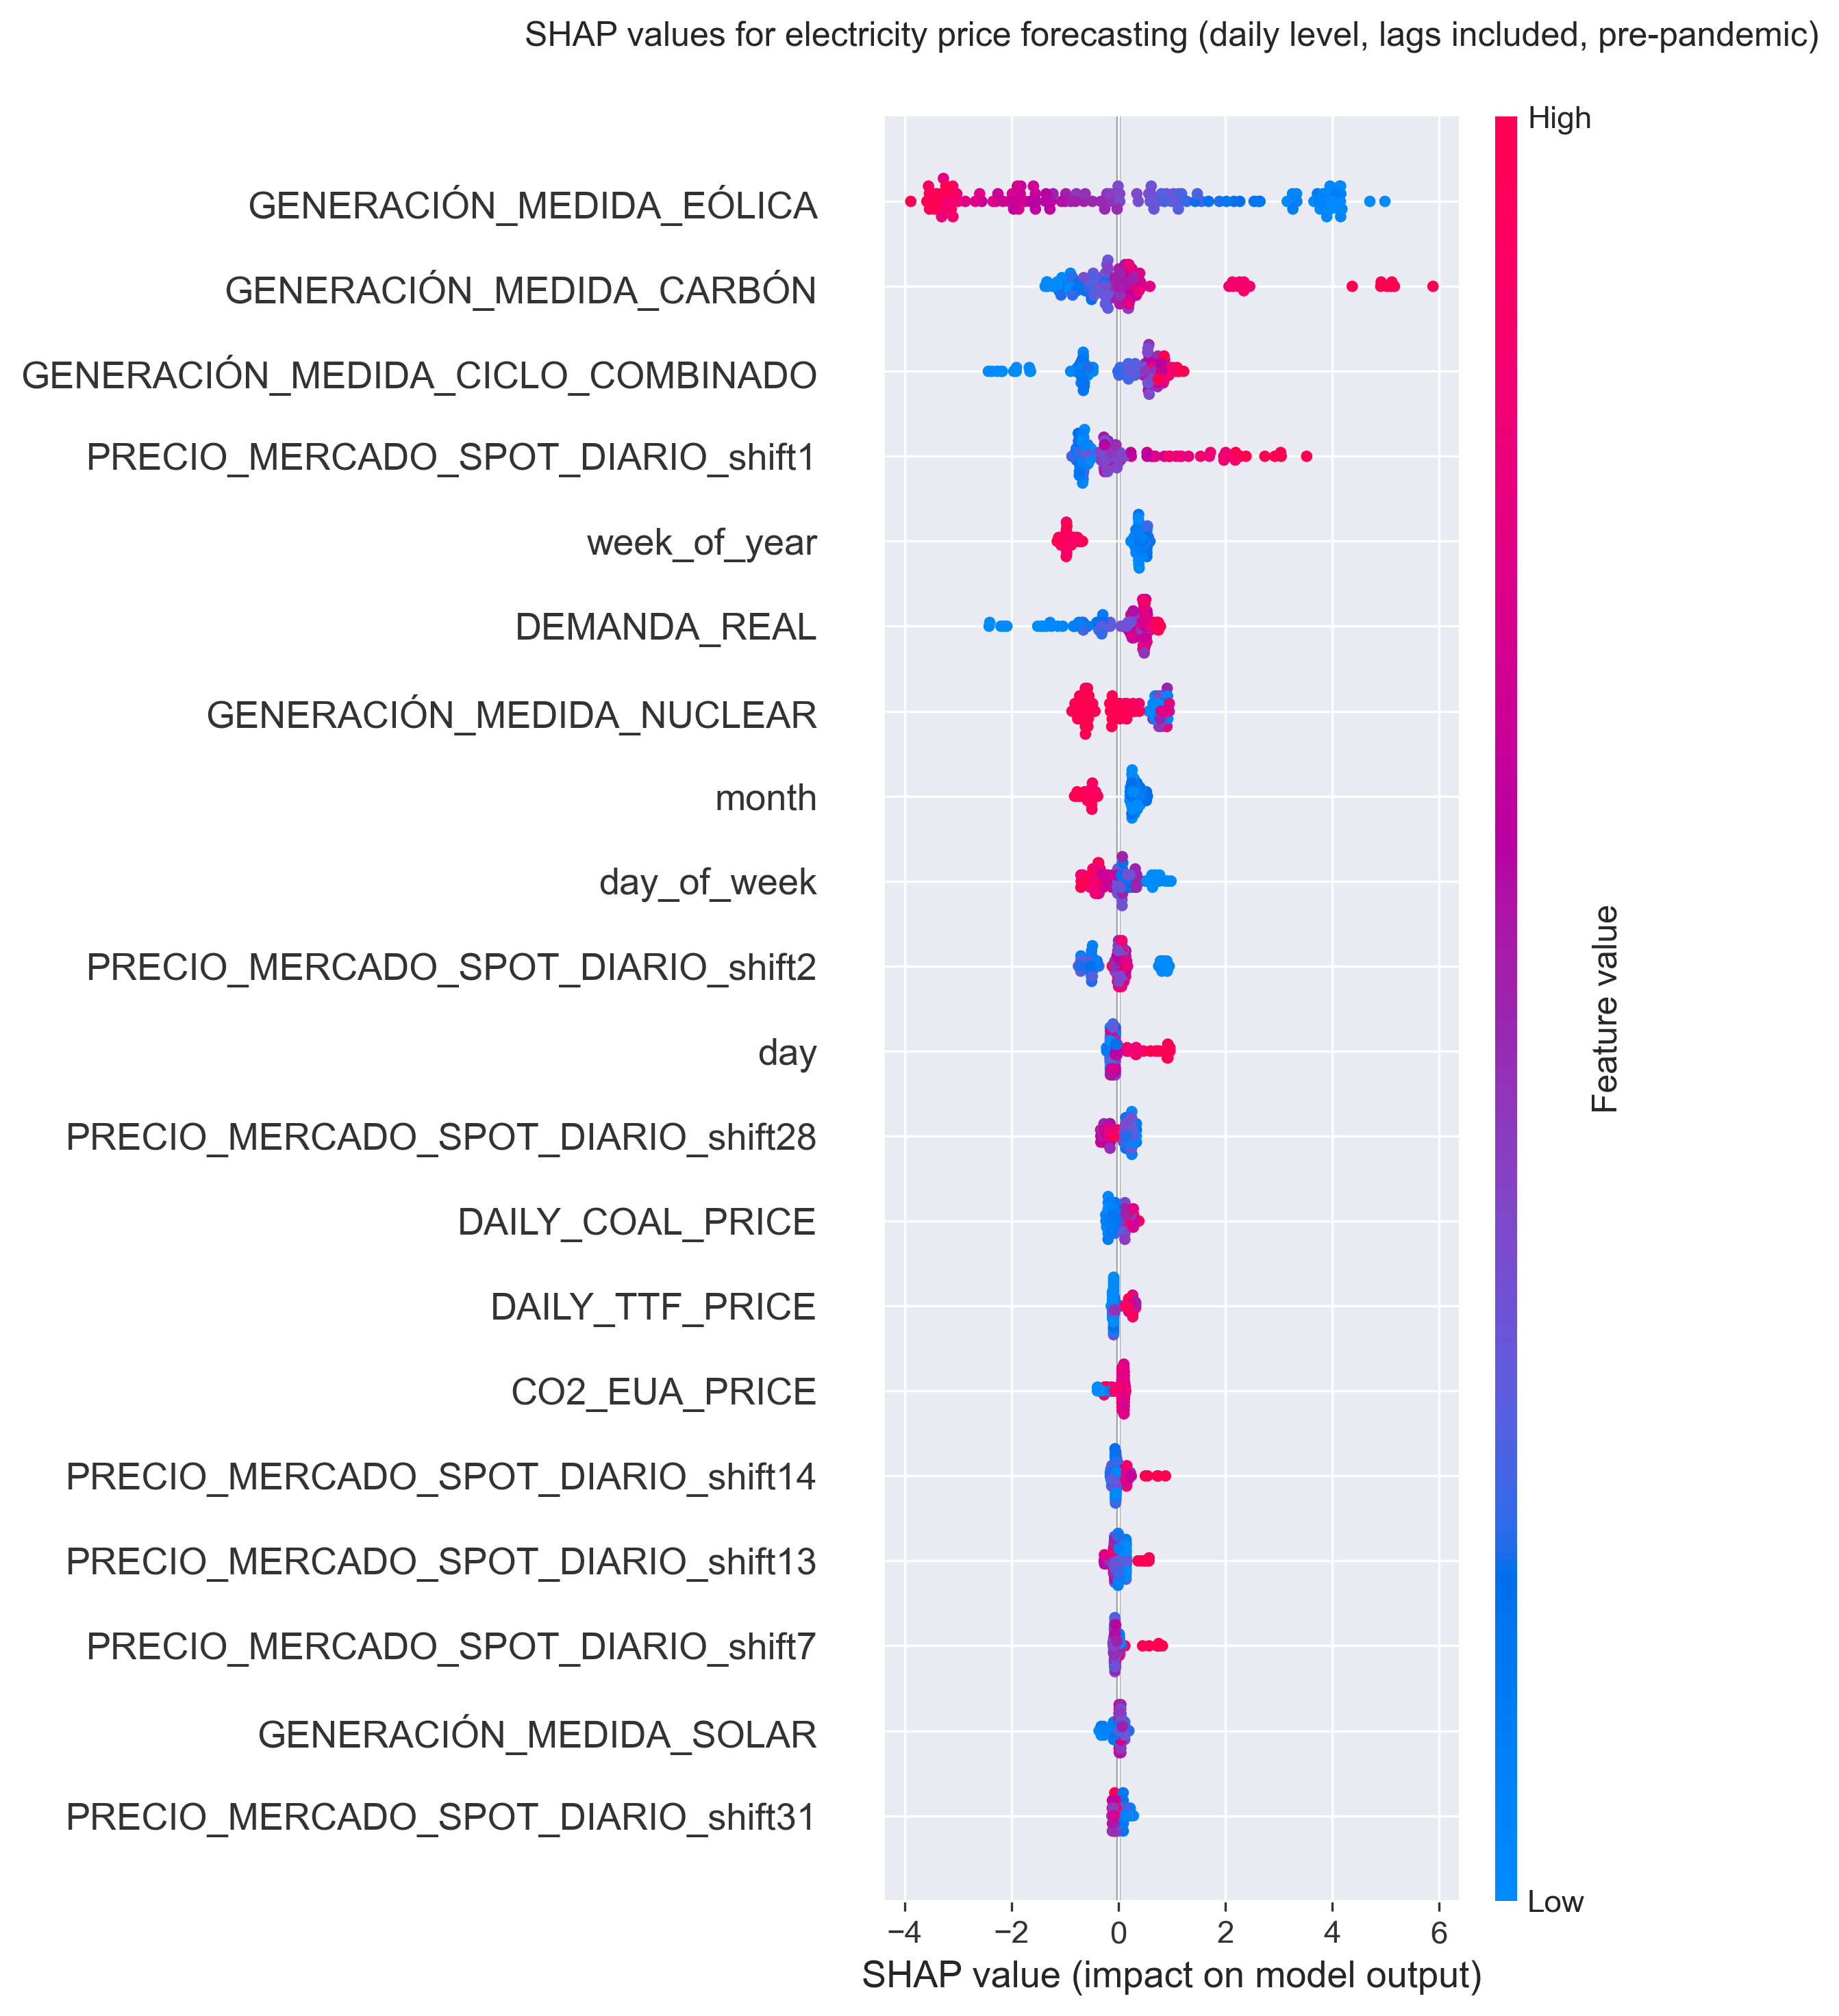
\includegraphics[width=0.7\linewidth]{images/analysis/shap-daily-pre}
    \caption{SHAP values for the daily pre-pandemic energy price forecasting.}
    \label{fig:shap-daily-pre}
\end{figure}


\subsection{After-Ukraine war scenario}
Let's now explore the after-war scenario. Data in use ranges from 2021-04-01 to 2023-03-31, and the best performing model changes to RF as seen in Table \ref{tab:cv-daily-post}.

\begin{table}[H]
\centering
\begin{tabular}{@{}l|l|l@{}}
\toprule
Model & MASE  & Modelling time (s)  \\ \midrule
RF    & 1.936 & 104.51  \\
GBT   & 2.153 & 67.30   \\
kNN   & 2.334 & 140.16  \\ \bottomrule
\end{tabular}
\caption{Model performance comparison trained over the daily post-war energy price.}
\label{tab:cv-daily-post}
\end{table}

After training RF with the complete cross-validation data and assessing the performance over the test partition, the MASE obtained is of 1.585. The result is shown in Figure \ref{fig:forecast-daily-post}. Nevertheless, if we inspect the prediction intervals, we see that they are much broader than in the pre-pandemic case.

\begin{figure}[H]
\centering
    \caption{Final forecasting of daily post-war energy price.}
    \label{fig:forecast-daily-post}
    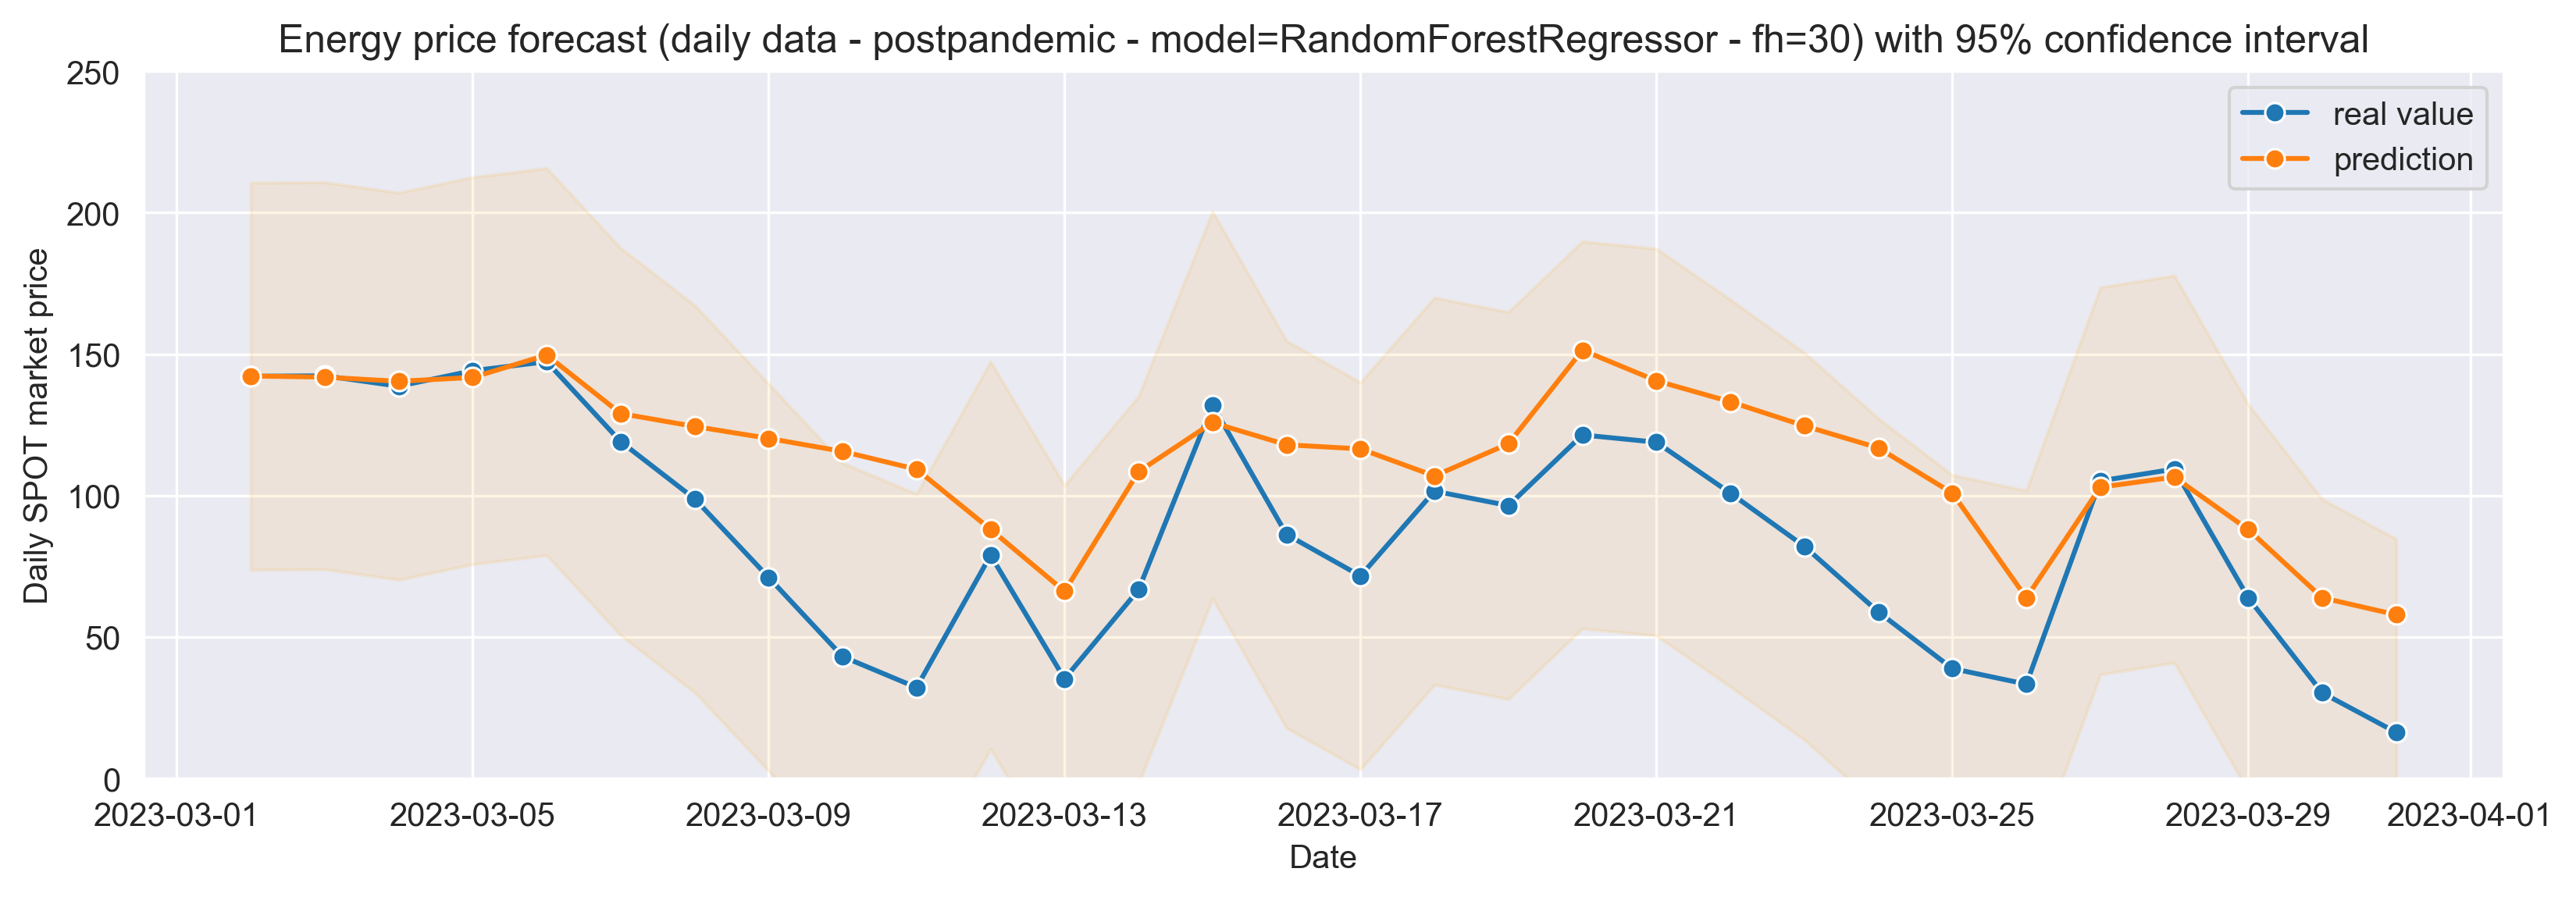
\includegraphics[scale=0.4]{images/analysis/forecast-daily-post}
\end{figure}

Again, lag 1 is the most influencing lag in Figure \ref{fig:shap-daily-post}. Now, hydropower generation appears in the top and is not helping to reduce energy price, but making it more expensive. Coal and combined cycle are still present in the top. TTF daily price also appears in the top, something that wasn't happening before, but its influence is not very clear.

\begin{figure}[H]
\centering
    \centering
    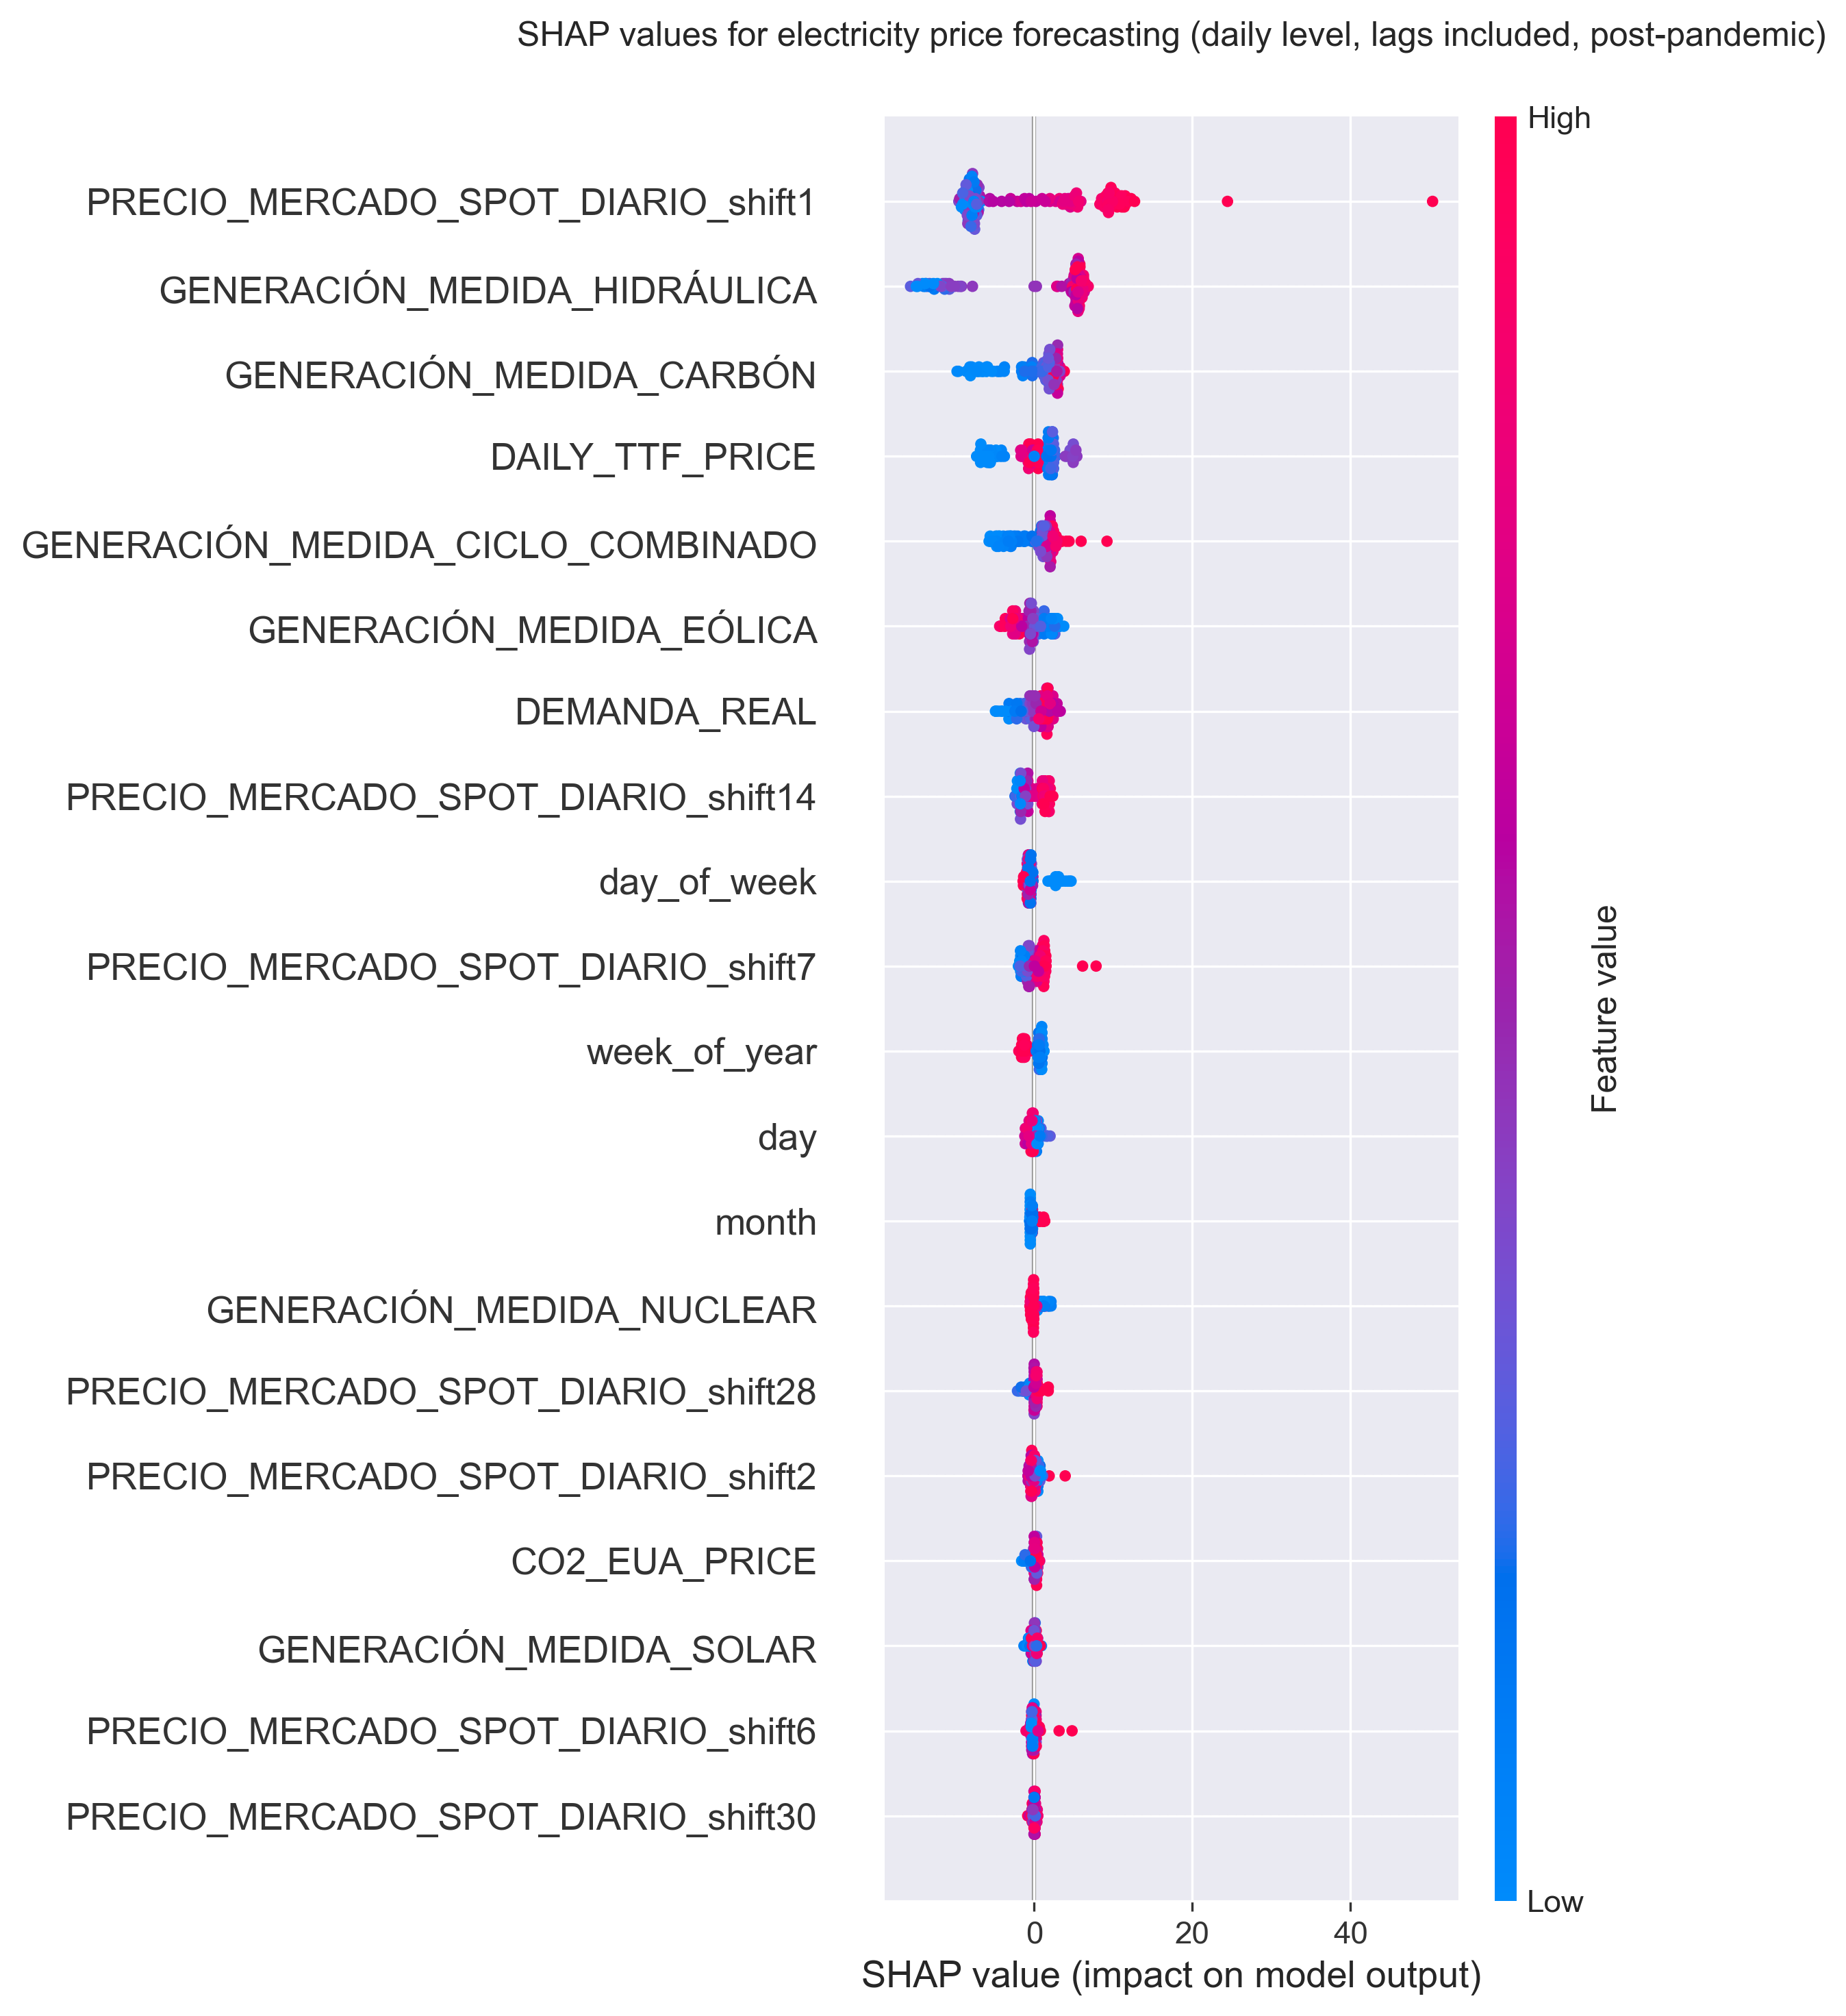
\includegraphics[width=0.7\linewidth]{images/analysis/shap-daily-post}
    \caption{SHAP values for the daily post-war energy price forecasting.}
    \label{fig:shap-daily-post}
\end{figure}

\subsection{Result discussion}

The best performing models are still those based in decision trees, GBT in the first scenario and RF in the second. As can be seen, again, the forecast in the post-war scenario seems to have more uncertainty.

The conclusions relative to SHAP values are similar for prices before the pandemic and after the war. In both cases, wind power contributes to lower the electricity price, while technologies based in commodities and hydropower tend to increase it. Newly added predictors such as gas or coal prices seem to not affect the forecast so much.

\newpage
\section{Monthly analysis}
In the monthly level the author won't compare pre-pandemic with post-war markets as there are no enough datapoints. He will perform the study over the complete series, with data from 2014-01 to 2023-03.

\noindent The same predictors as before are used, except those related with date, that change:
\begin{itemize}
    \item \textbf{Date predictors:} Month and year.
\end{itemize}

Cross-validation will be performed using 12 windows and step size 1, while the forecasting horizon will consist of 12 months. The best performing model in this case is GBT, obtaining a MASE of 1.69 in Table \ref{tab:cv-monthly}.

\begin{table}[H]
\centering
\begin{tabular}{@{}l|l|l@{}}
\toprule
Model & MASE  & Modelling time (s)  \\ \midrule
GBT   & 1.690  & 84.55    \\
RF    & 1.749  & 117.03   \\
kNN   & 2.662  & 108.33   \\ \bottomrule
\end{tabular}
\caption{}
\label{tab:cv-monthly}
\end{table}

When applying holdout over the complete series, the obtained MASE grows up to 7.347, an indicator of the poor performance of the forecast. This can be verified in Figure \ref{fig:forecast-monthly}, in which the confidence intervals are broad. Why this increase with respect to cross-validation? Because now, the test partition falls on the 2022-2023 period, in which the market has changed and uncertainty is high due to Ukraine's war. On the other hand, in cross-validation, many testing folds fall before the price increase due to the war, so the testing and training partitions were sharing the same properties, making the forecast easier.

\begin{figure}[H]
\centering
    \caption{Final forecasting of monthly energy price.}
    \label{fig:forecast-monthly}
    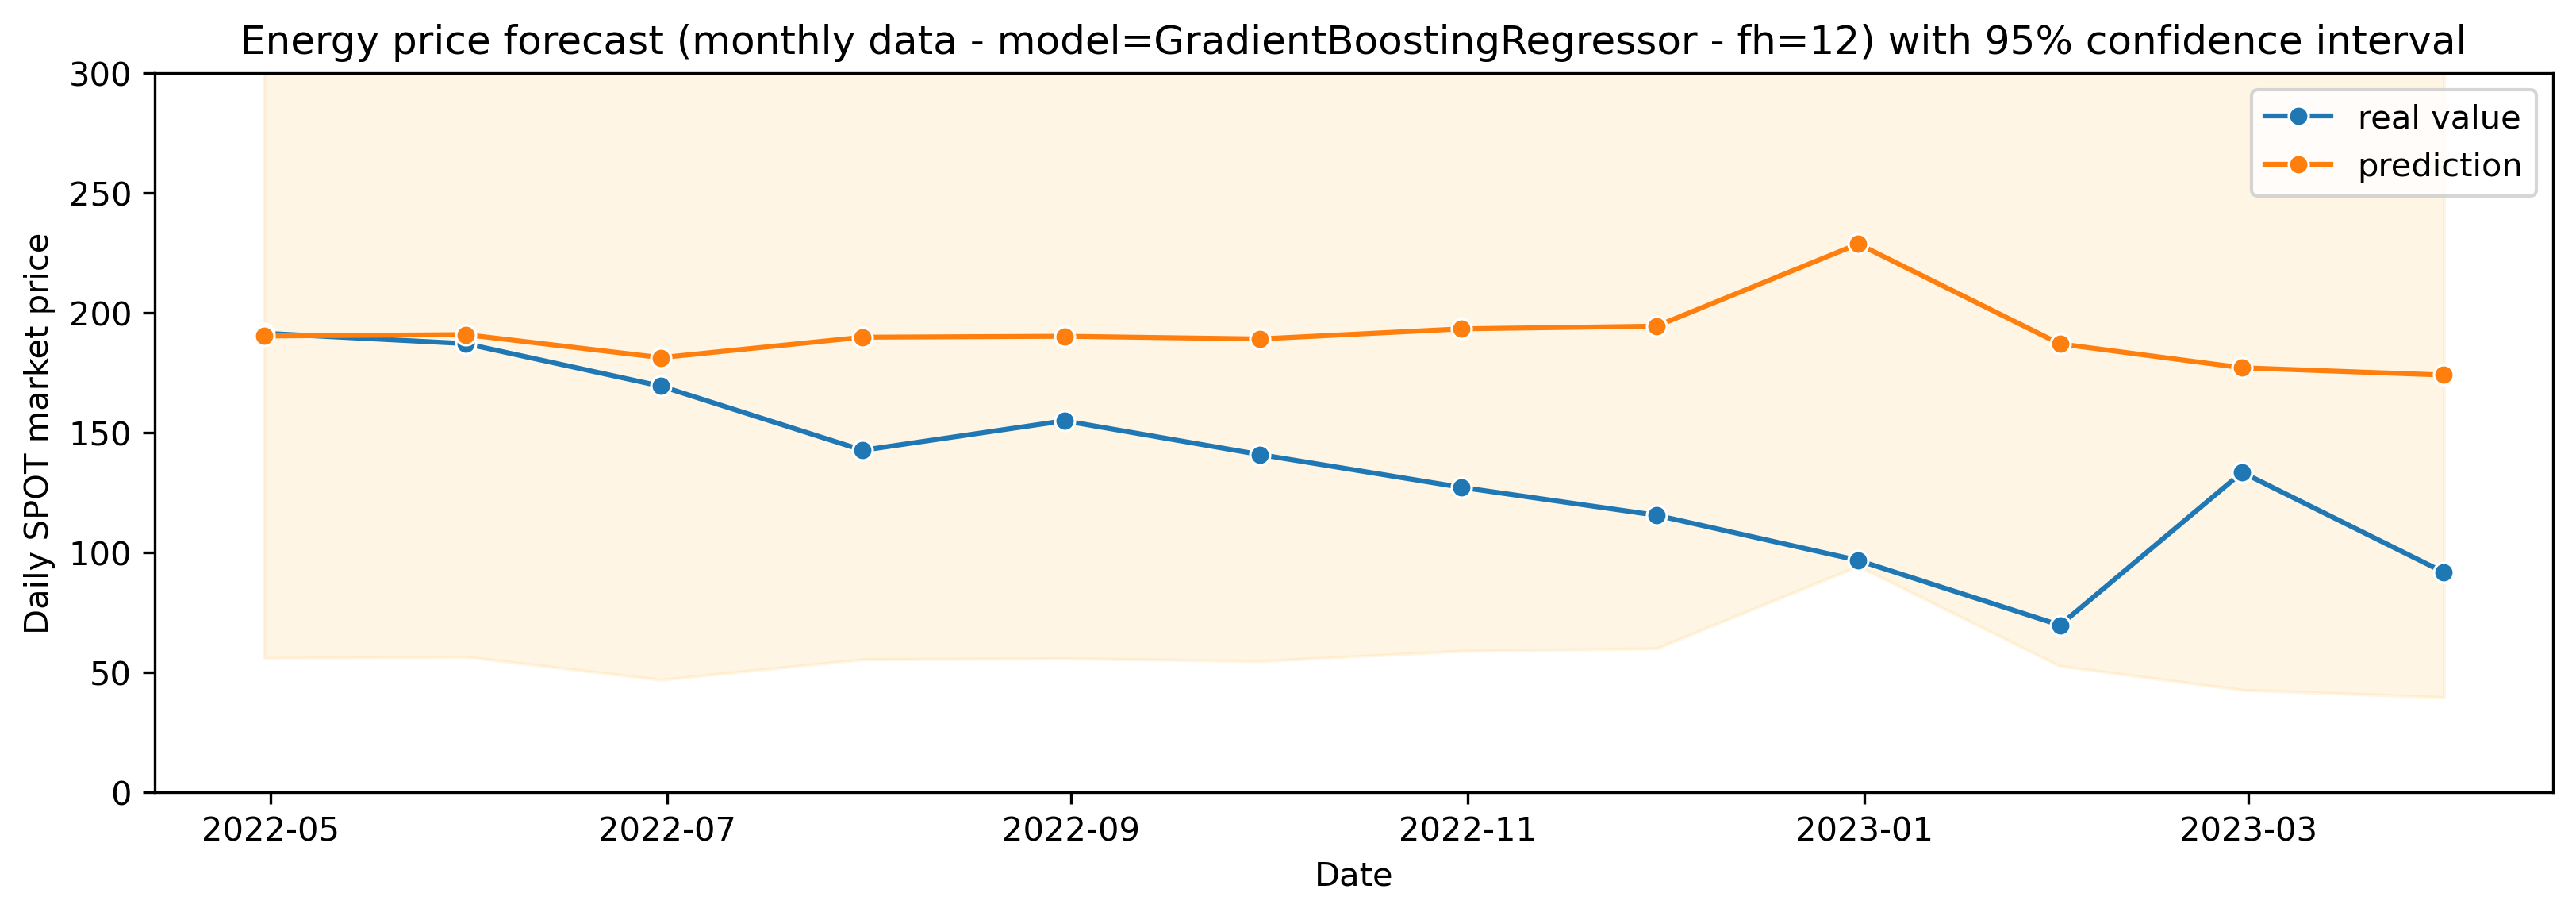
\includegraphics[scale=0.4]{images/analysis/forecast-monthly}
\end{figure}

In view of the low forecasting performance, the SHAP values should be taken with a grain of salt. In fact, the results in Figure \ref{fig:shap-monthly} don't make sense: the use of solar generation is increasing prices, while coal generation is lowering them. We won't consider this SHAP values as valid, as probably the models is not learning due to the lack of datapoints.

\begin{figure}[H]
\centering
    \centering
    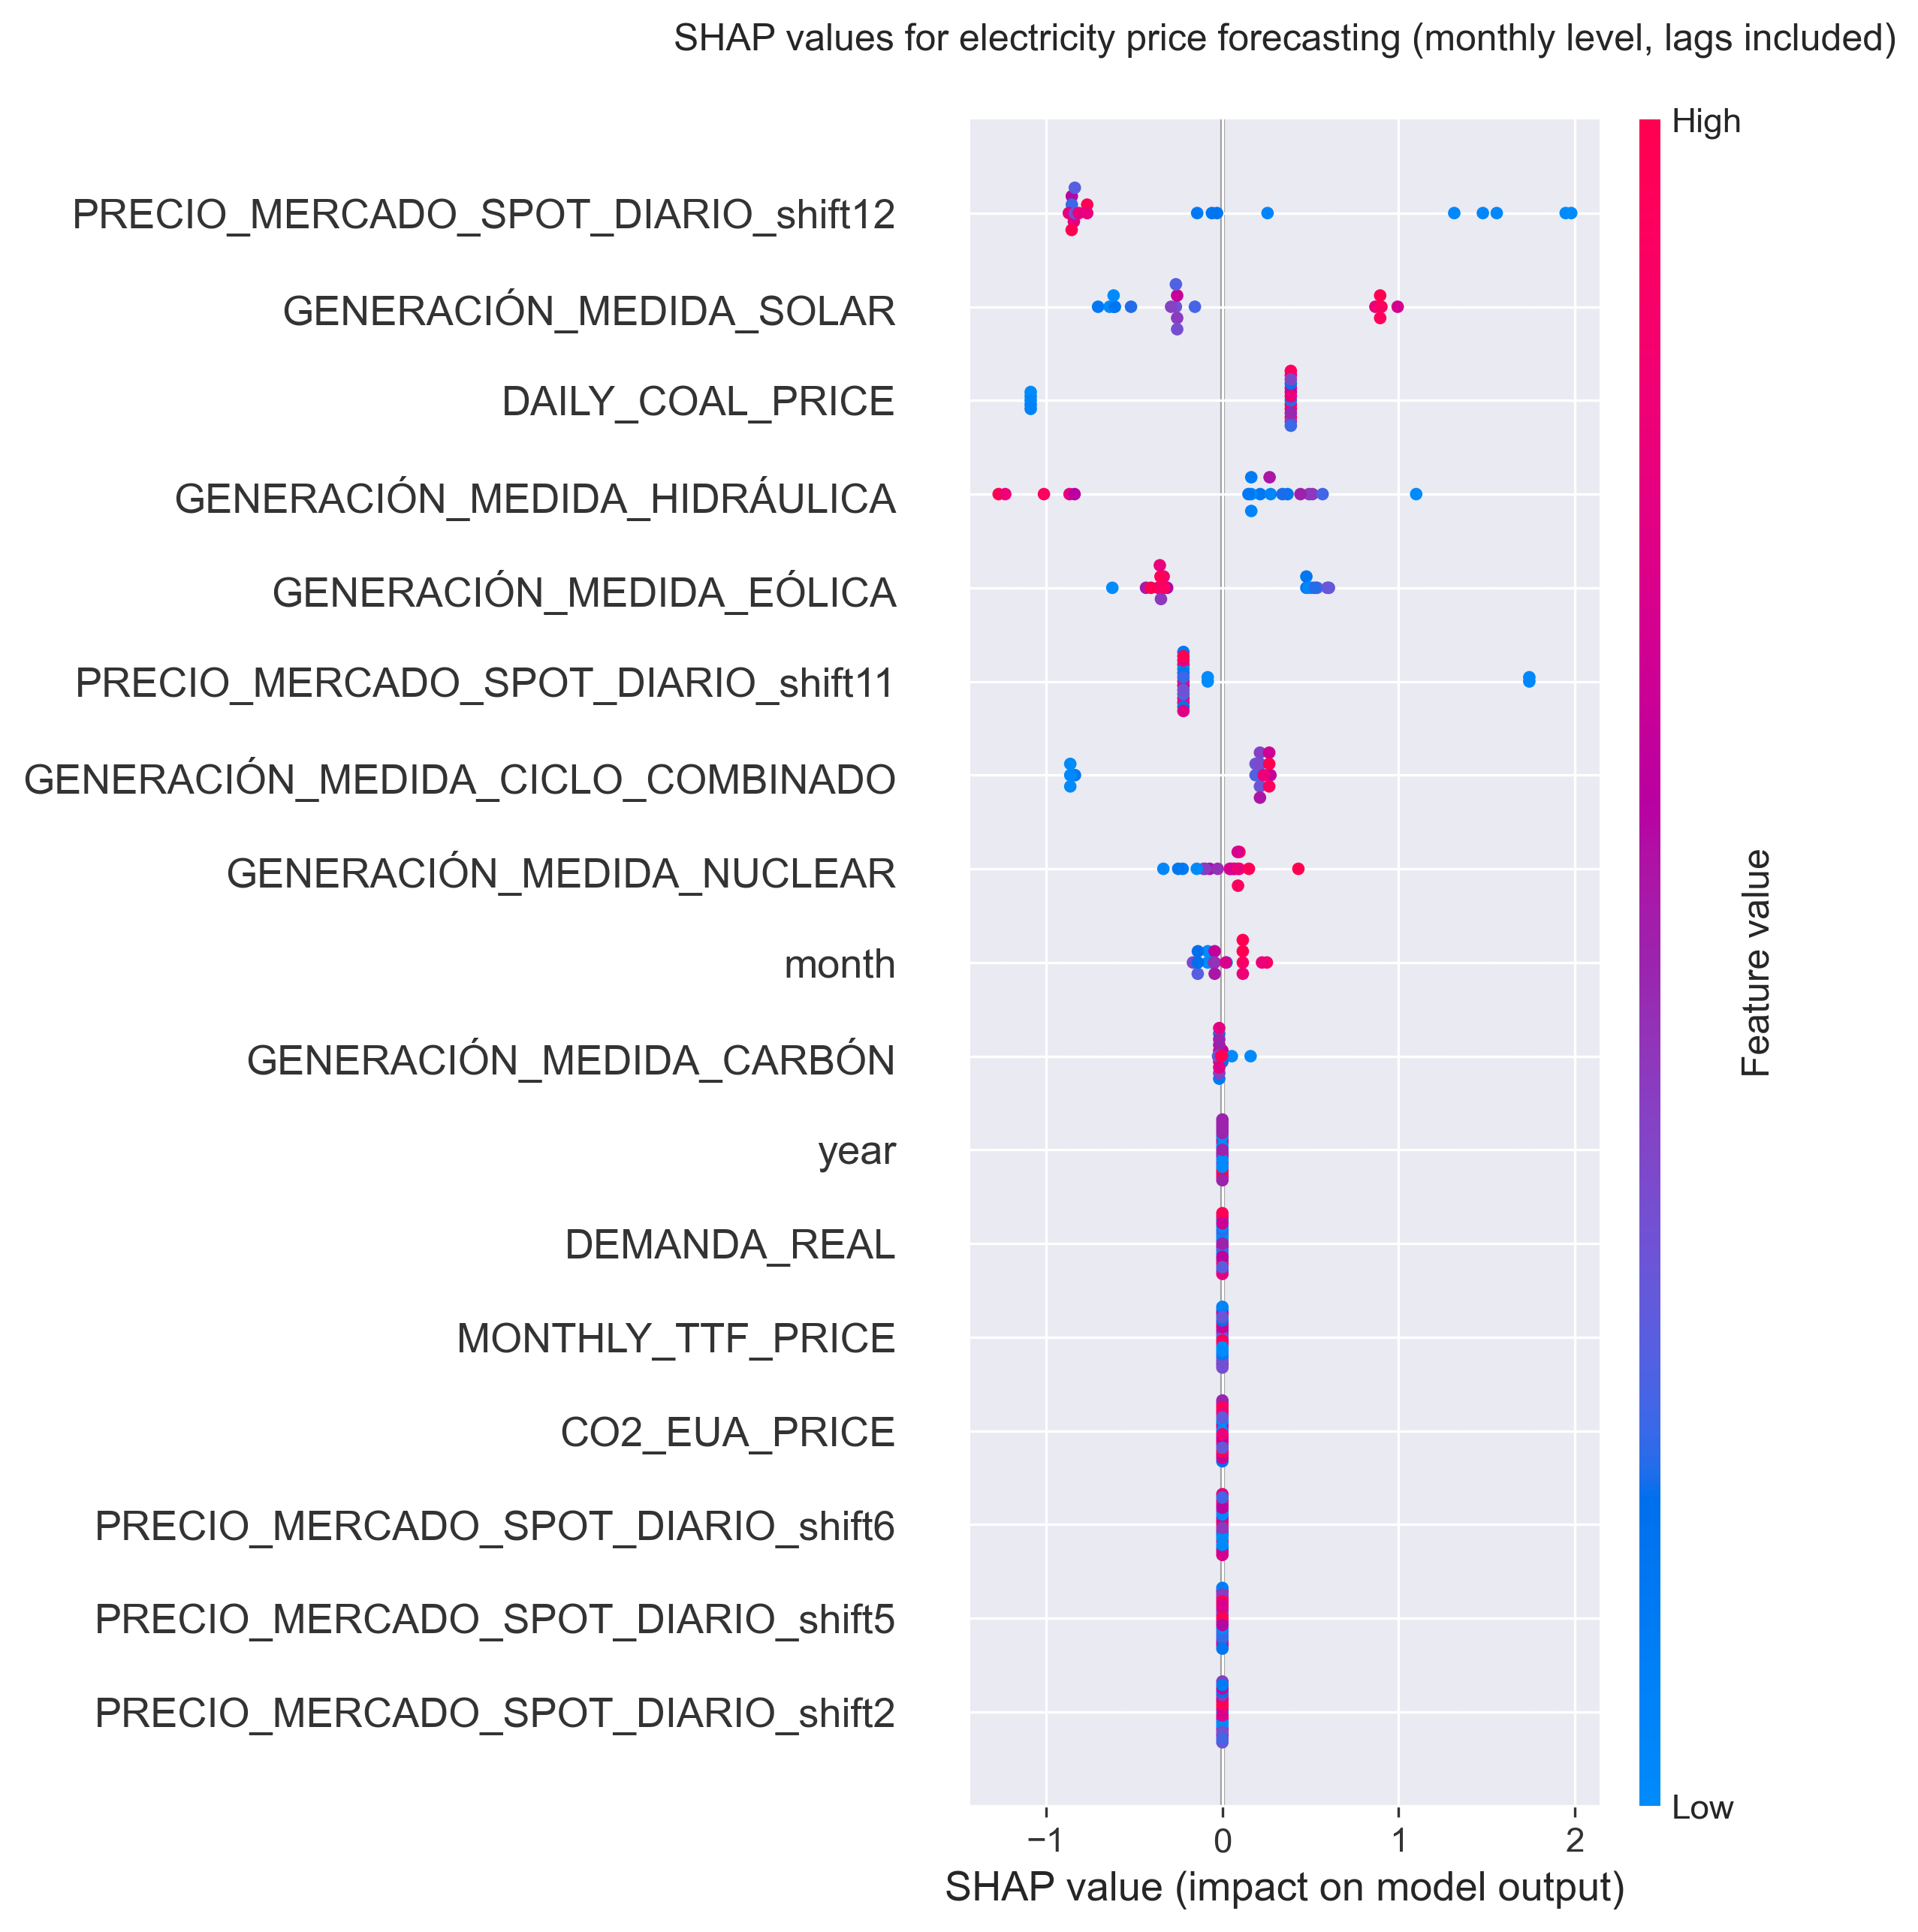
\includegraphics[width=0.7\linewidth]{images/analysis/shap-monthly}
    \caption{SHAP values for the monthly energy price forecasting.}
    \label{fig:shap-monthly}
\end{figure}

\newpage
\section{Yearly analysis}

If data is aggregated by year, there are no enough datapoints to model the series. That's why the author will just perform a descriptive analysis. In Figure \ref{fig:spot-yearly}, the electricity price series is shown: it can be seen how it has remained below 100 euros per megawatt for many years, until 2021.

\begin{figure}[H]
\centering
    \centering
    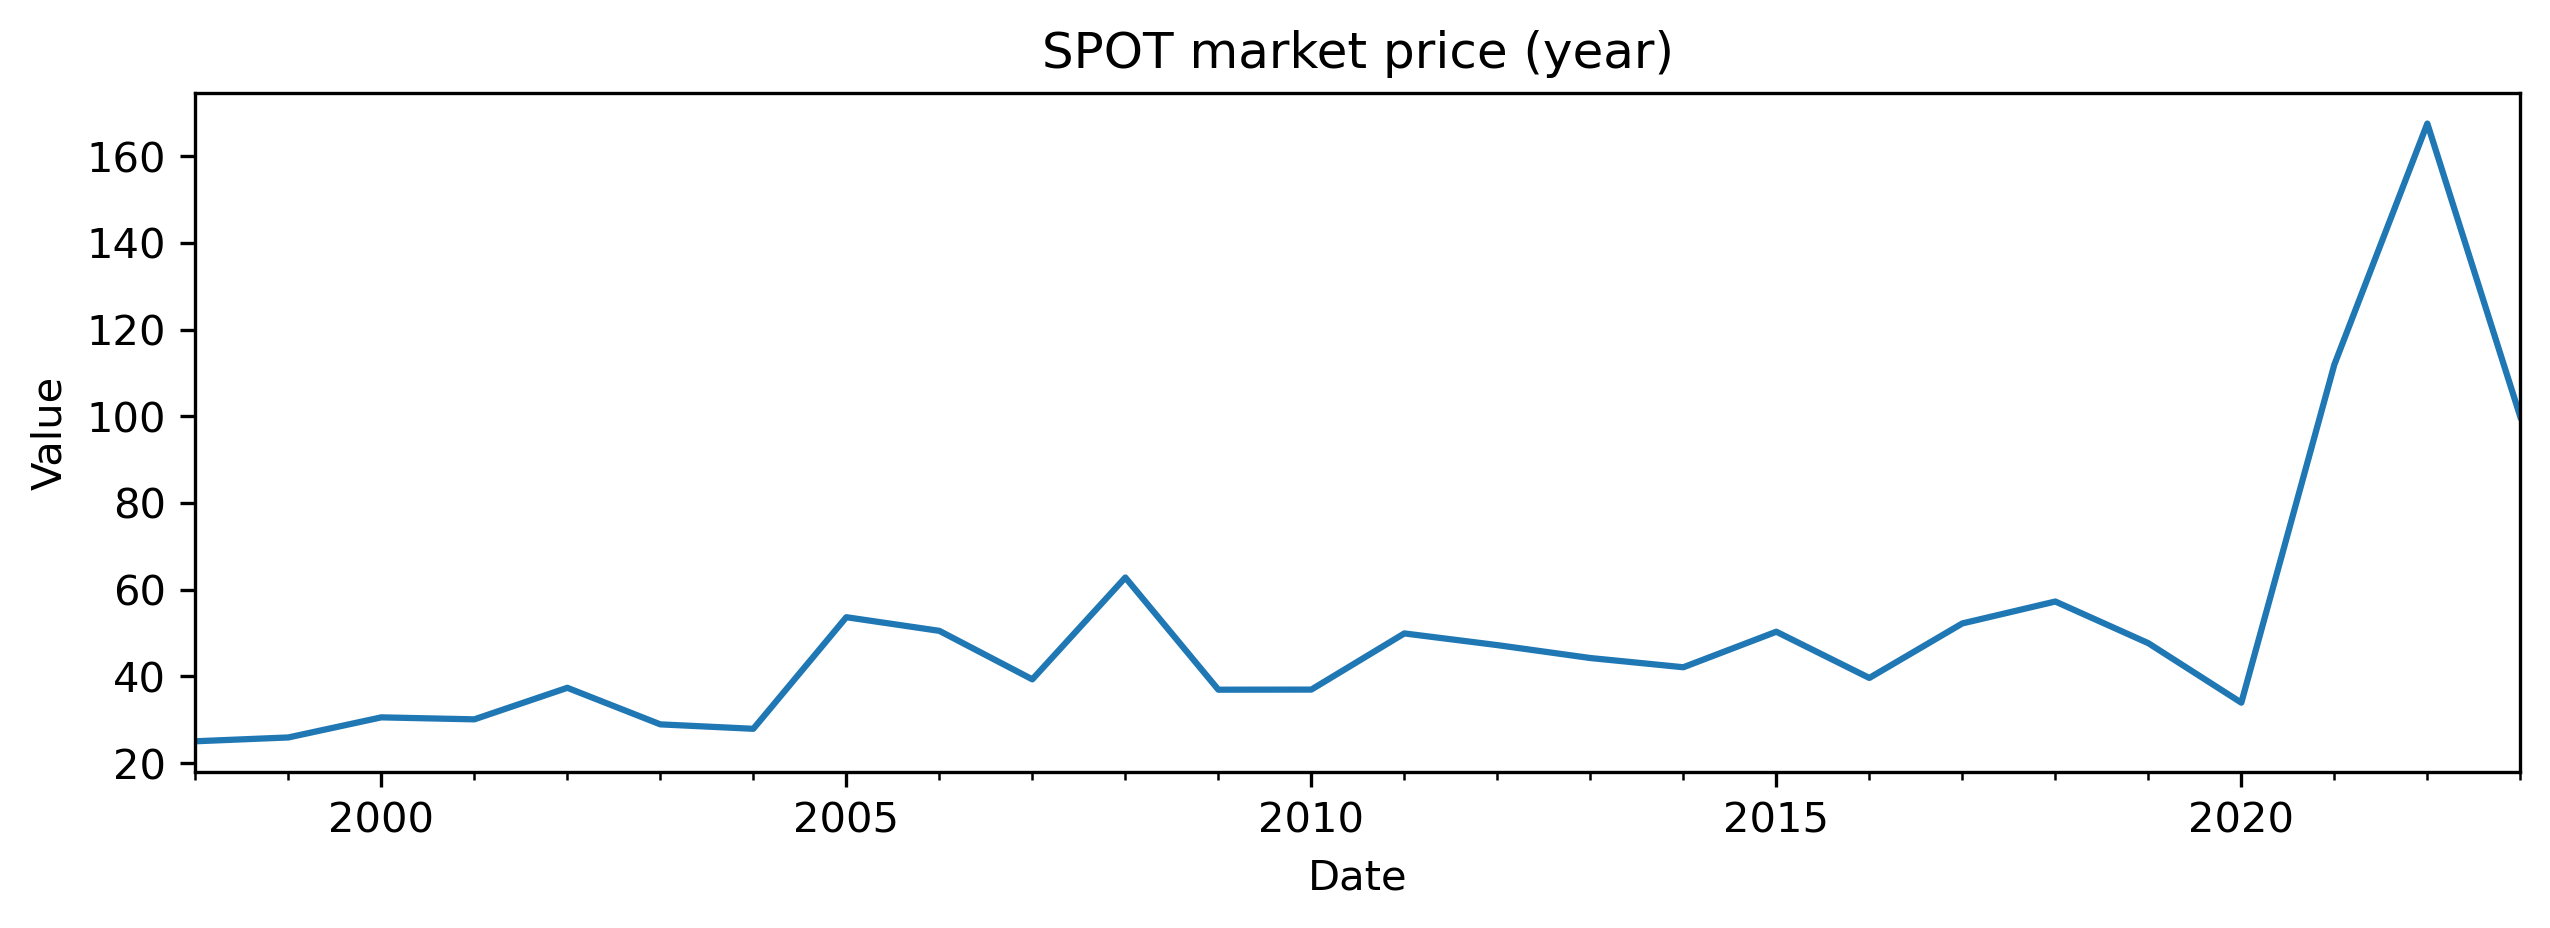
\includegraphics[width=0.7\linewidth]{images/analysis/spot-yearly}
    \caption{Electricity market SPOT price aggregated by year.}
    \label{fig:spot-yearly}
\end{figure}

The war in Ukraine made the gas price go up. Russia decreased gas flow to Europe, making it a scarce commodity and driving up its price. If we check TTF's gas index price curve in Figure \ref{fig:ttf-yearly}, it shows a similar behaviour to the electricity series. The same happens for ARGUS/McCloskey coal price index in Figure \ref{fig:coal-yearly}.

\begin{figure}[H]
\centering
    \begin{subfigure}{0.7\textwidth}
        \centering
        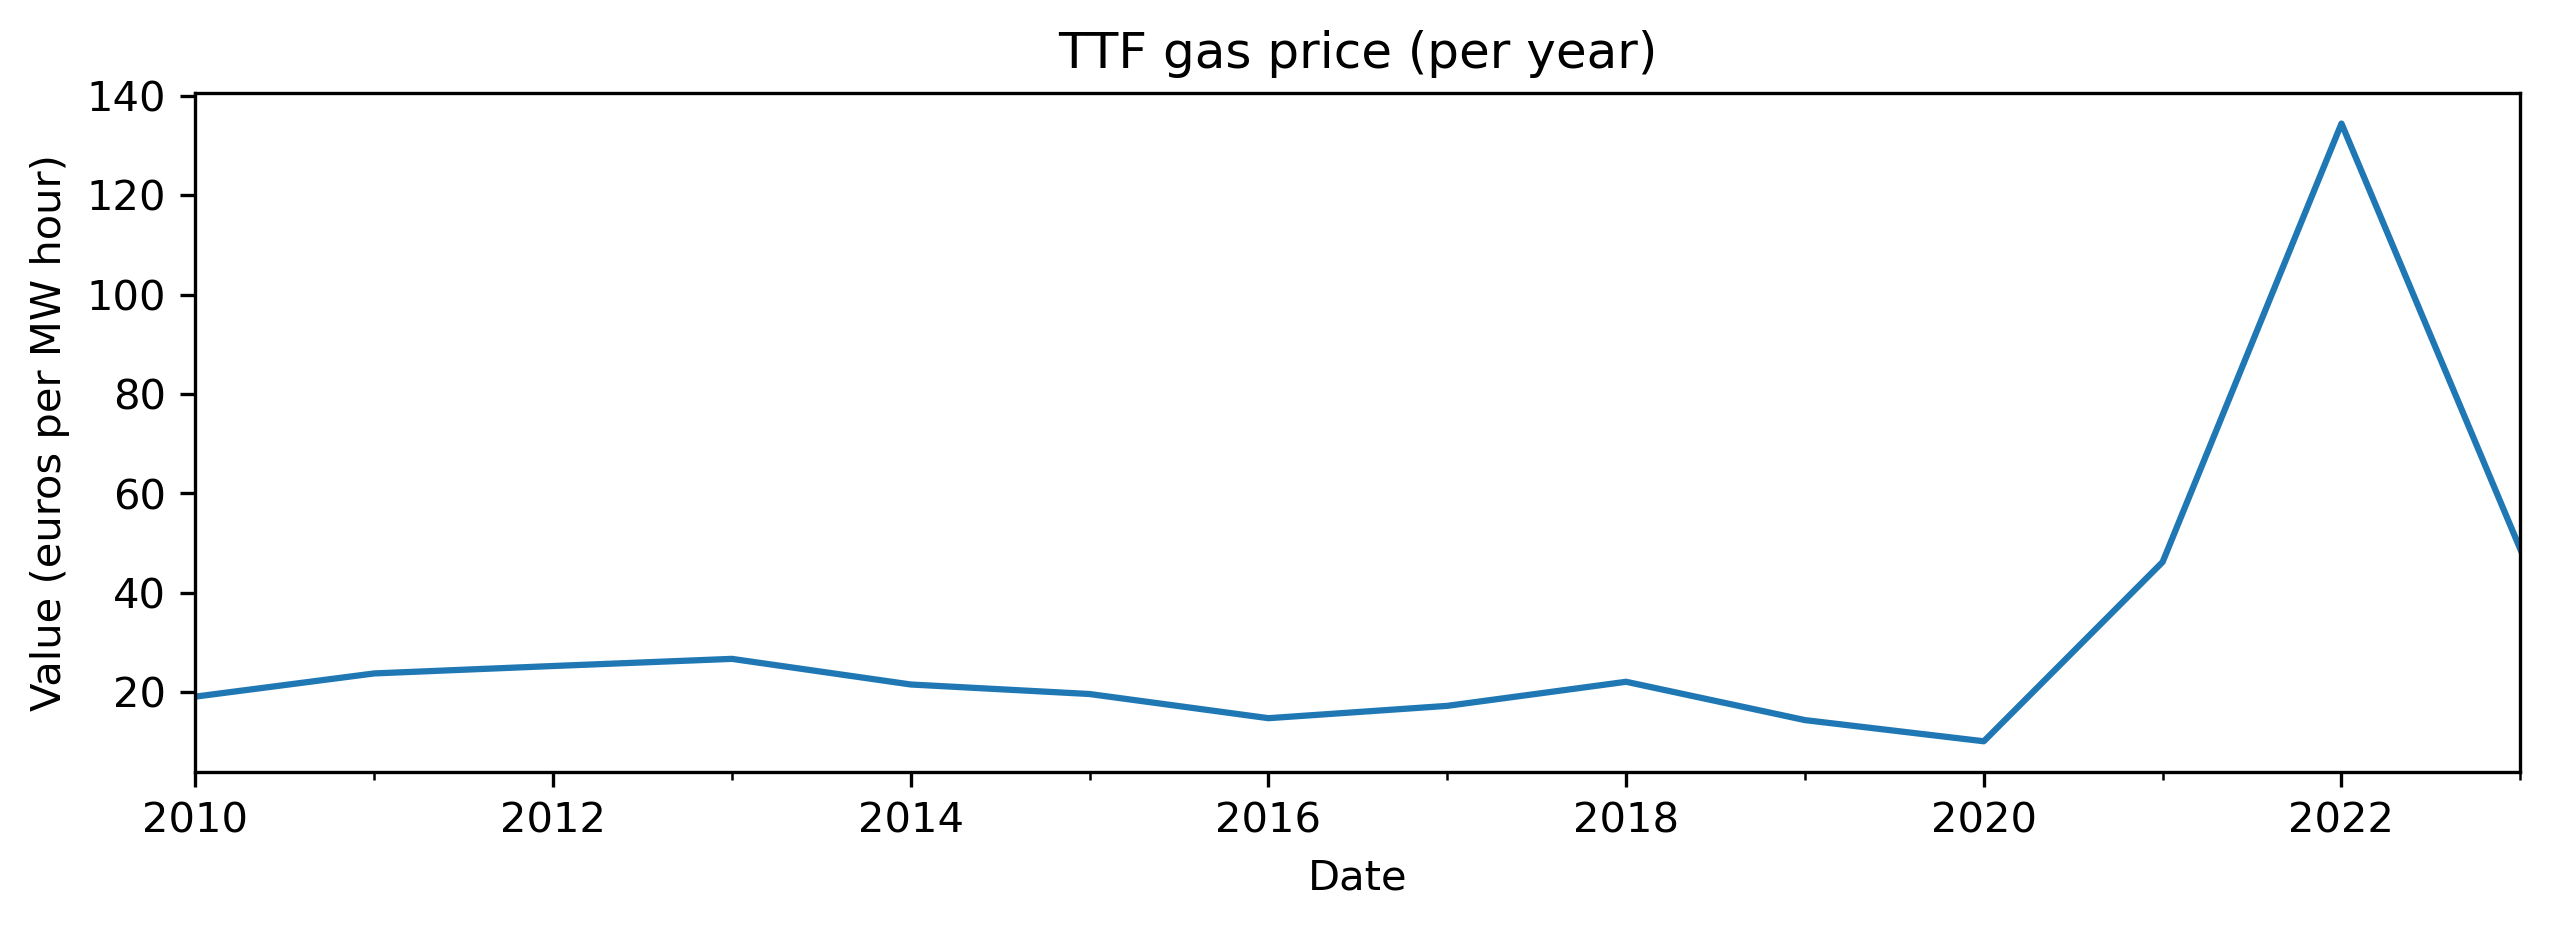
\includegraphics[width=1\linewidth]{images/analysis/ttf-yearly}
        \caption{TTF gas price series.}
        \label{fig:ttf-yearly}
    \end{subfigure}
\end{figure}

\begin{figure}[H]\ContinuedFloat
    \begin{subfigure}{0.7\textwidth}
        \centering
        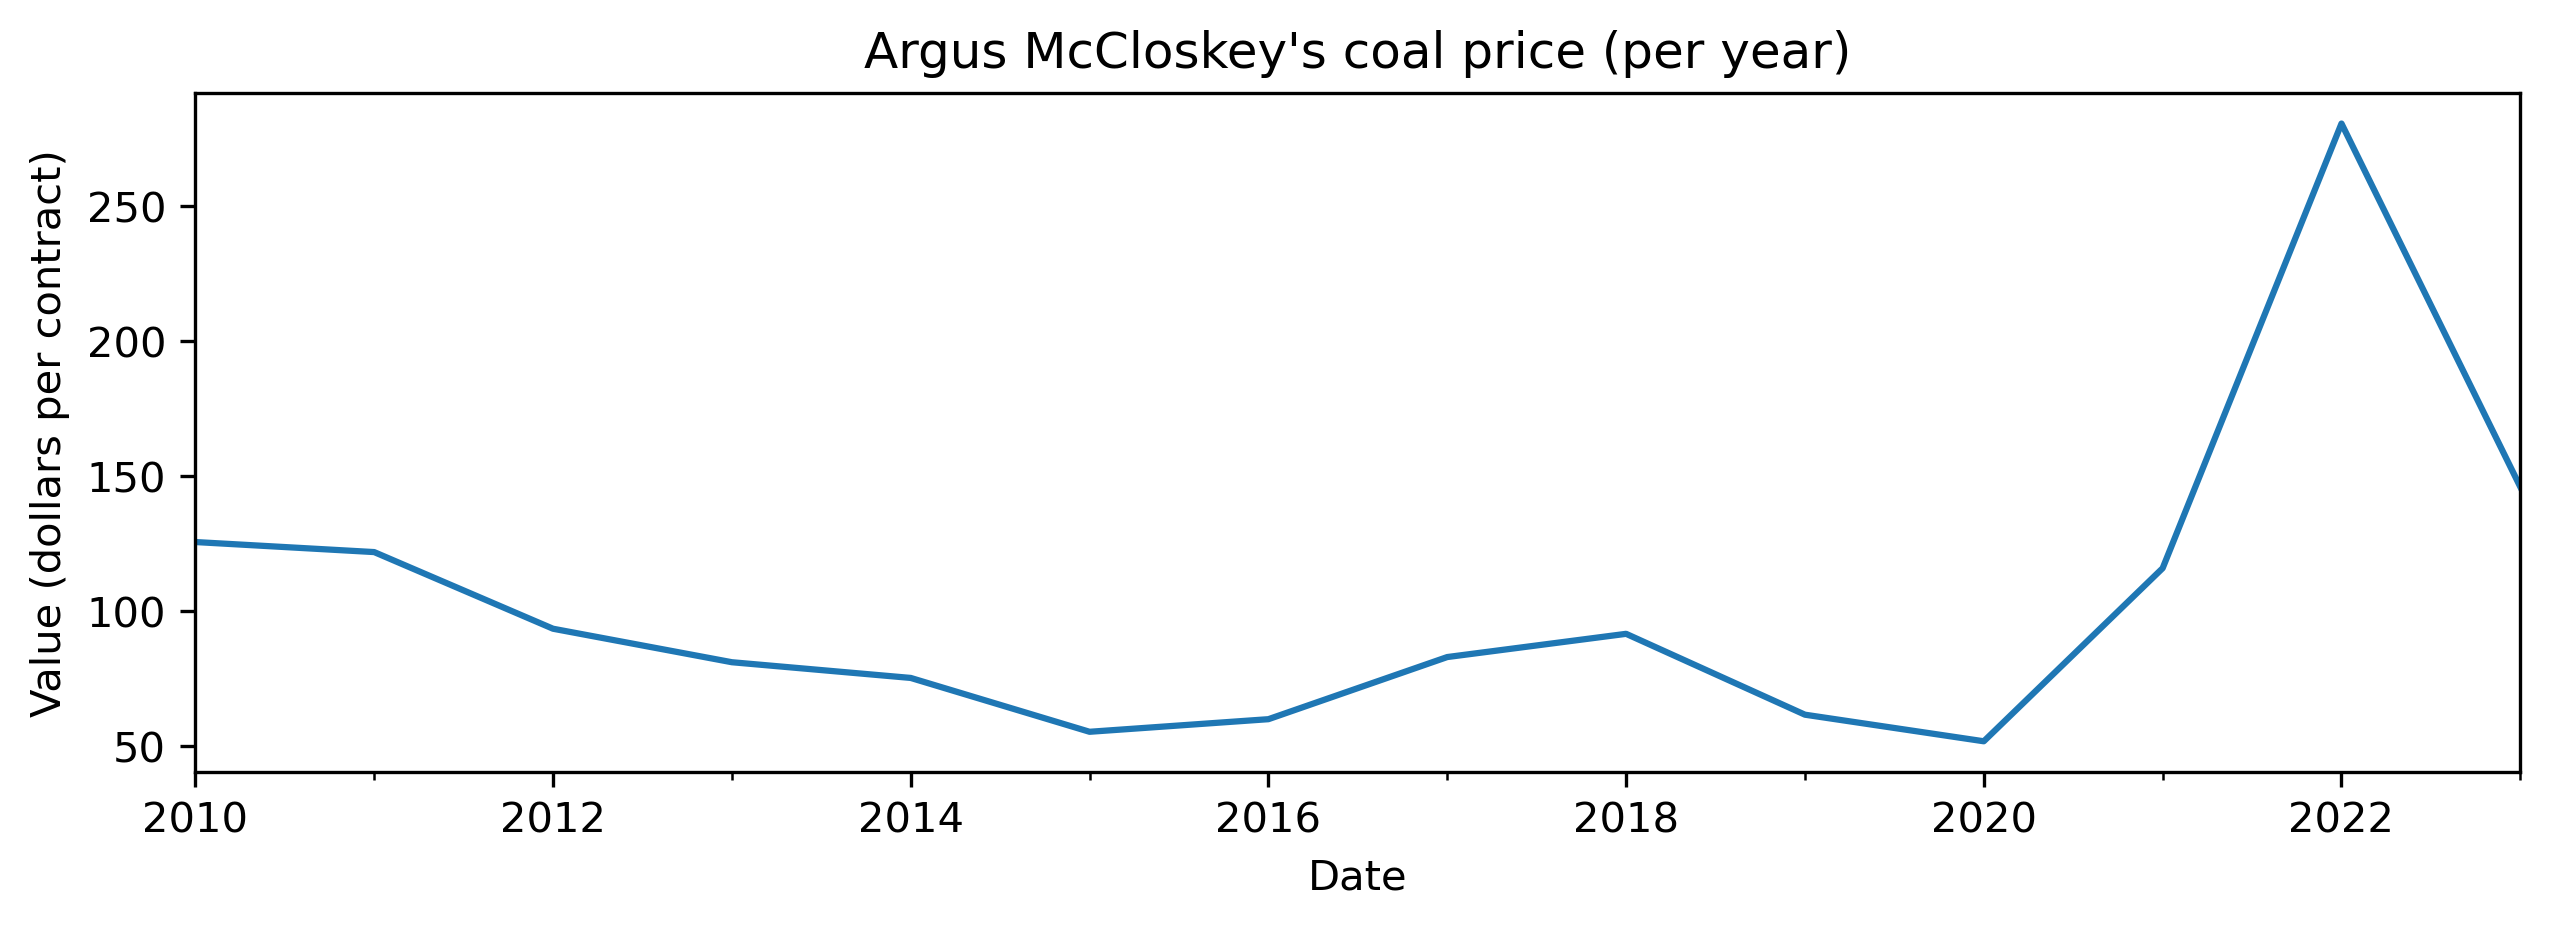
\includegraphics[width=1\linewidth]{images/analysis/coal-yearly}
        \caption{ARGUS/McCloskey coal price series.}
        \label{fig:coal-yearly}
    \end{subfigure}

    \caption{Commodities aggregated by year.}
    \label{fig:ttf-coal-yearly}
\end{figure}

This increase is what has specially made the prices go up, as commodity-based technologies are still relevant nowadays, specially gas. As can be seen in Figure \ref{fig:gen-yearly}, the use of combined cycle has increased in the previous years, although coal based generation has decreased.

\begin{figure}[H]
\centering
    \begin{subfigure}{.45\textwidth}
        \centering
        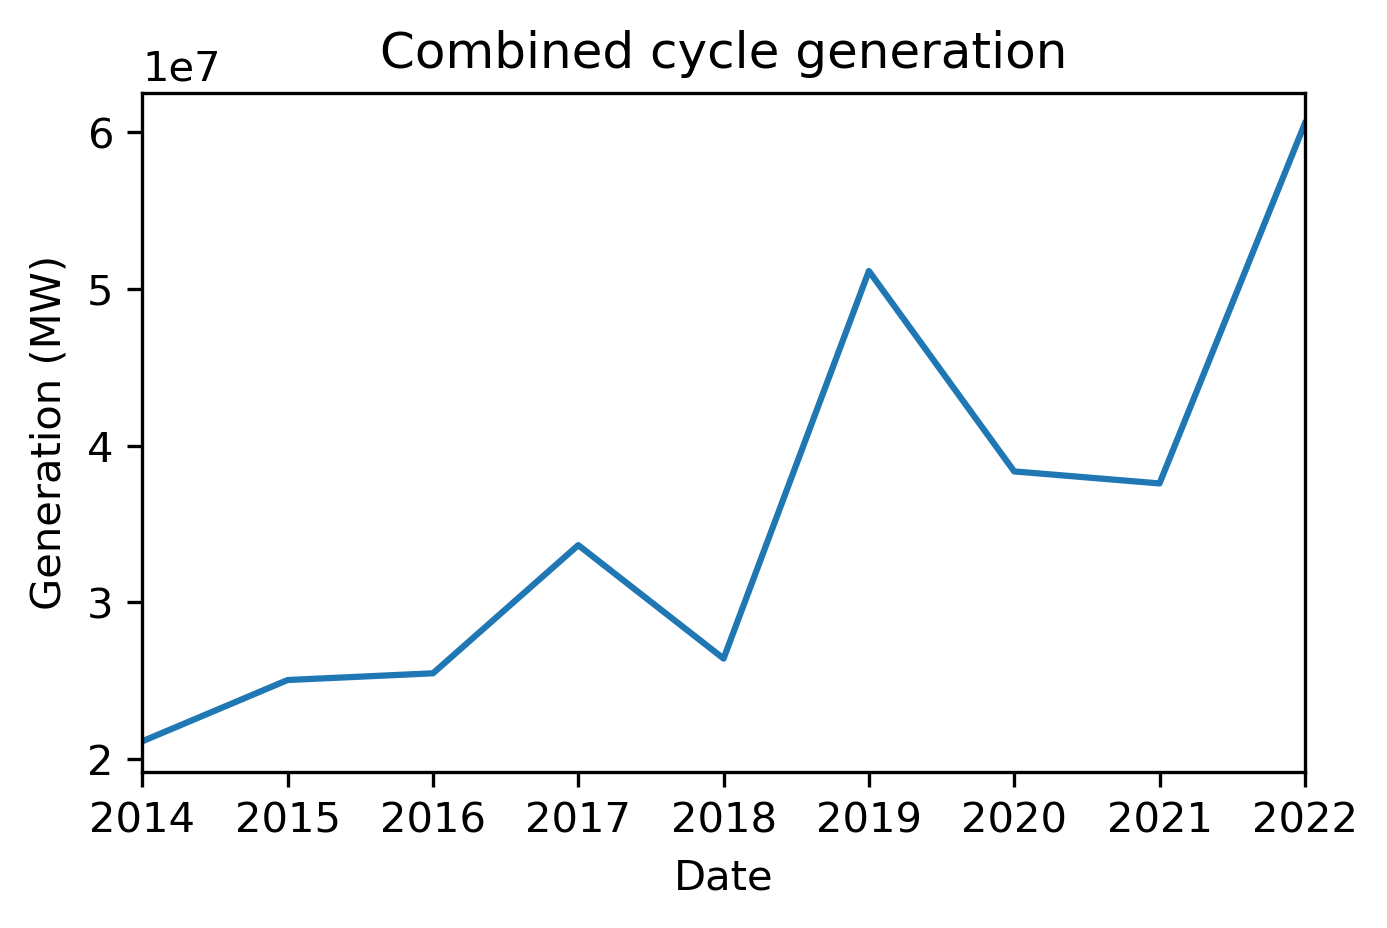
\includegraphics[width=1\linewidth]{images/analysis/comb-gen-yearly}
        \caption{Combined cycle generation}
    \end{subfigure}
    \begin{subfigure}{.45\textwidth}
        \centering
        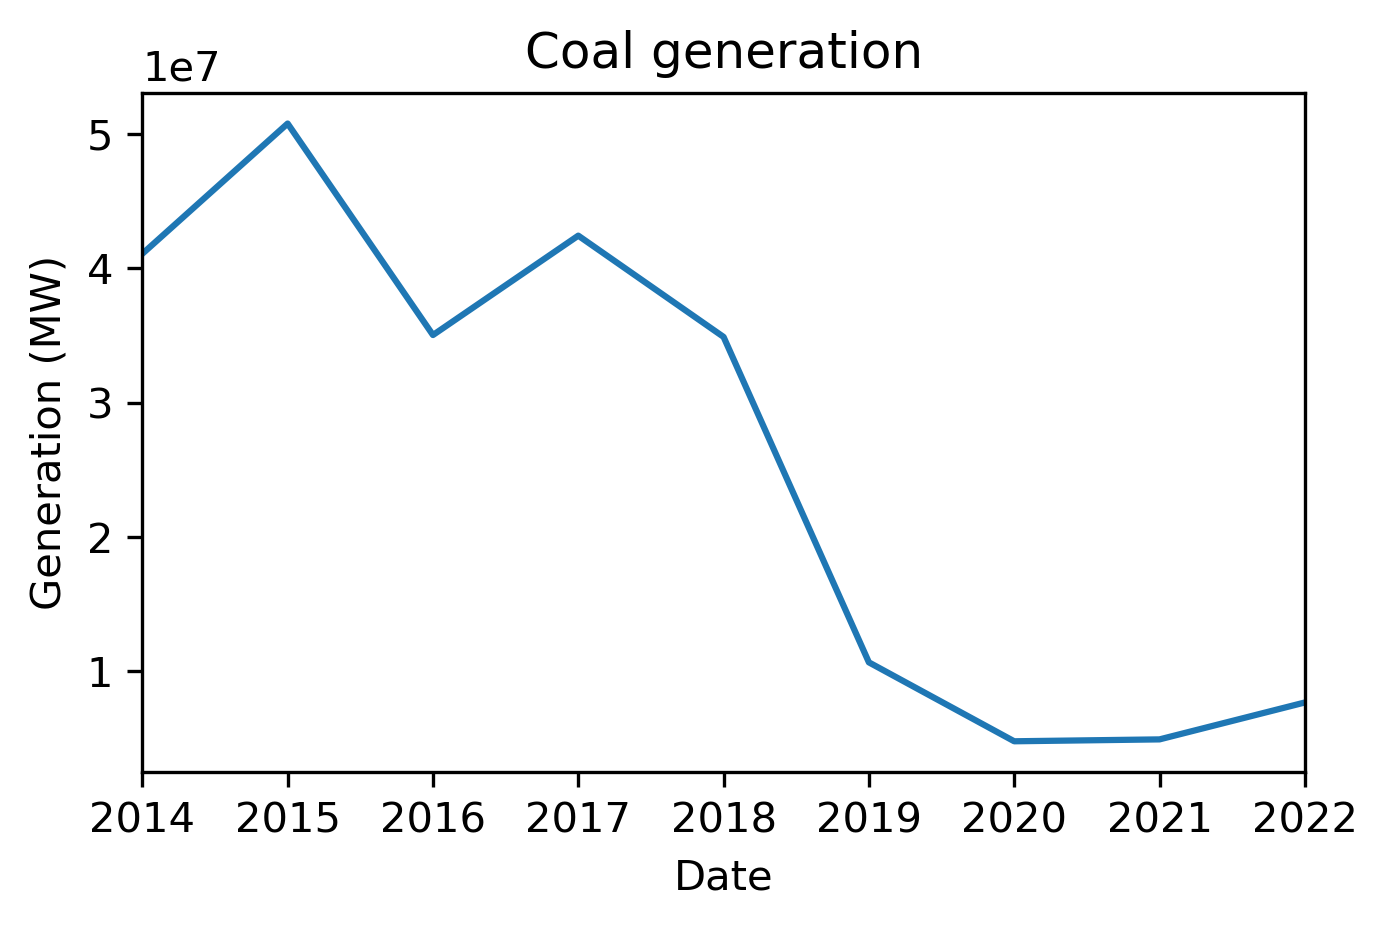
\includegraphics[width=1\linewidth]{images/analysis/coal-gen-yearly}
        \caption{Coal based generation}
    \end{subfigure}
\end{figure}

\begin{figure}[H]\ContinuedFloat
    \begin{subfigure}{.45\textwidth}
        \centering
        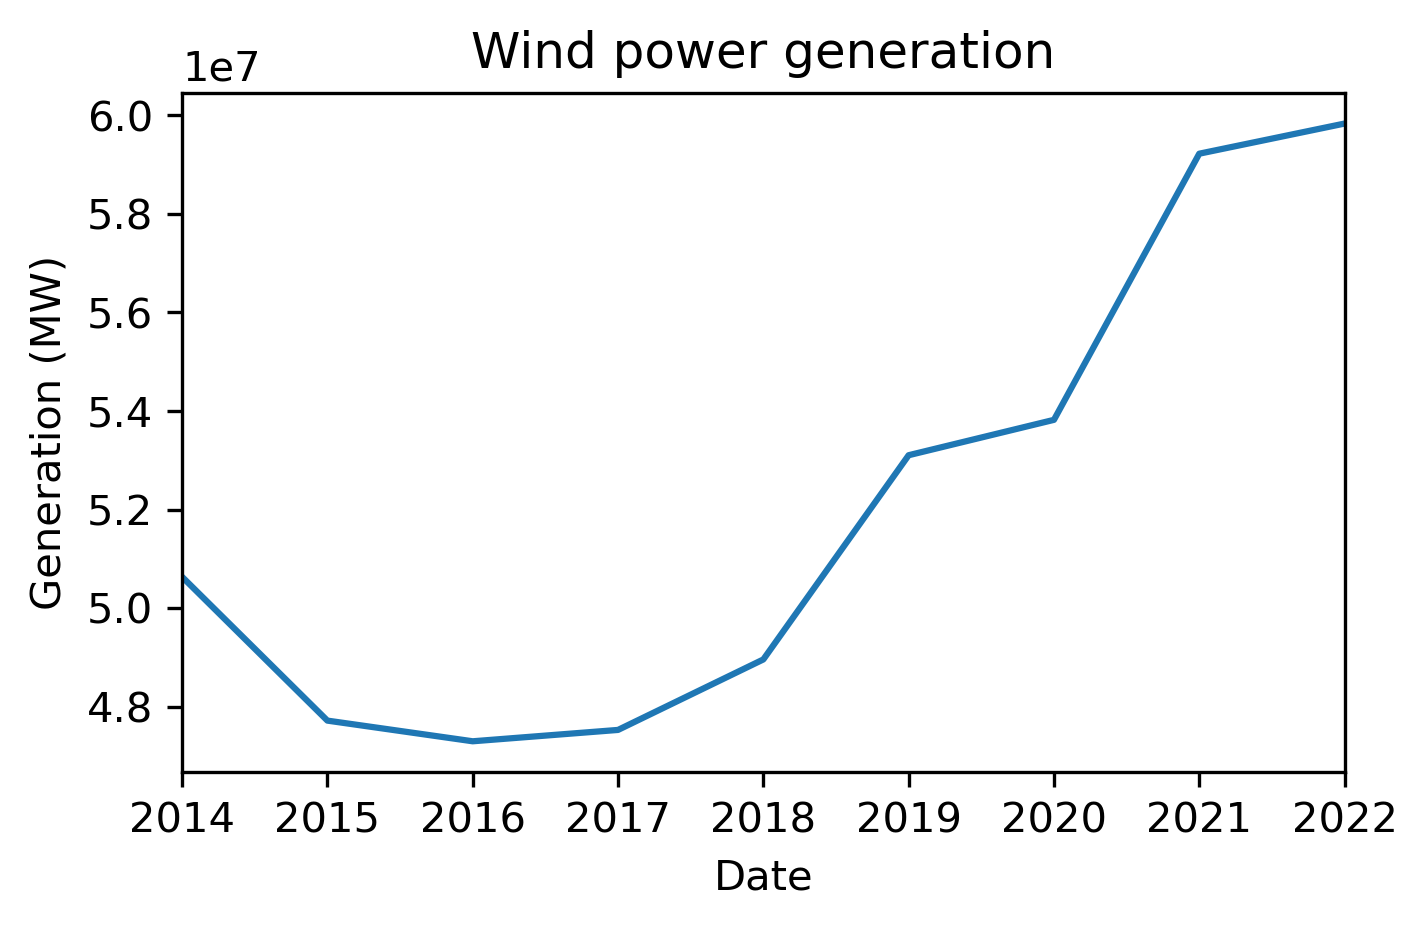
\includegraphics[width=1\linewidth]{images/analysis/wind-gen-yearly}
        \caption{Wind power generation}
    \end{subfigure}
    \begin{subfigure}{.45\textwidth}
        \centering
        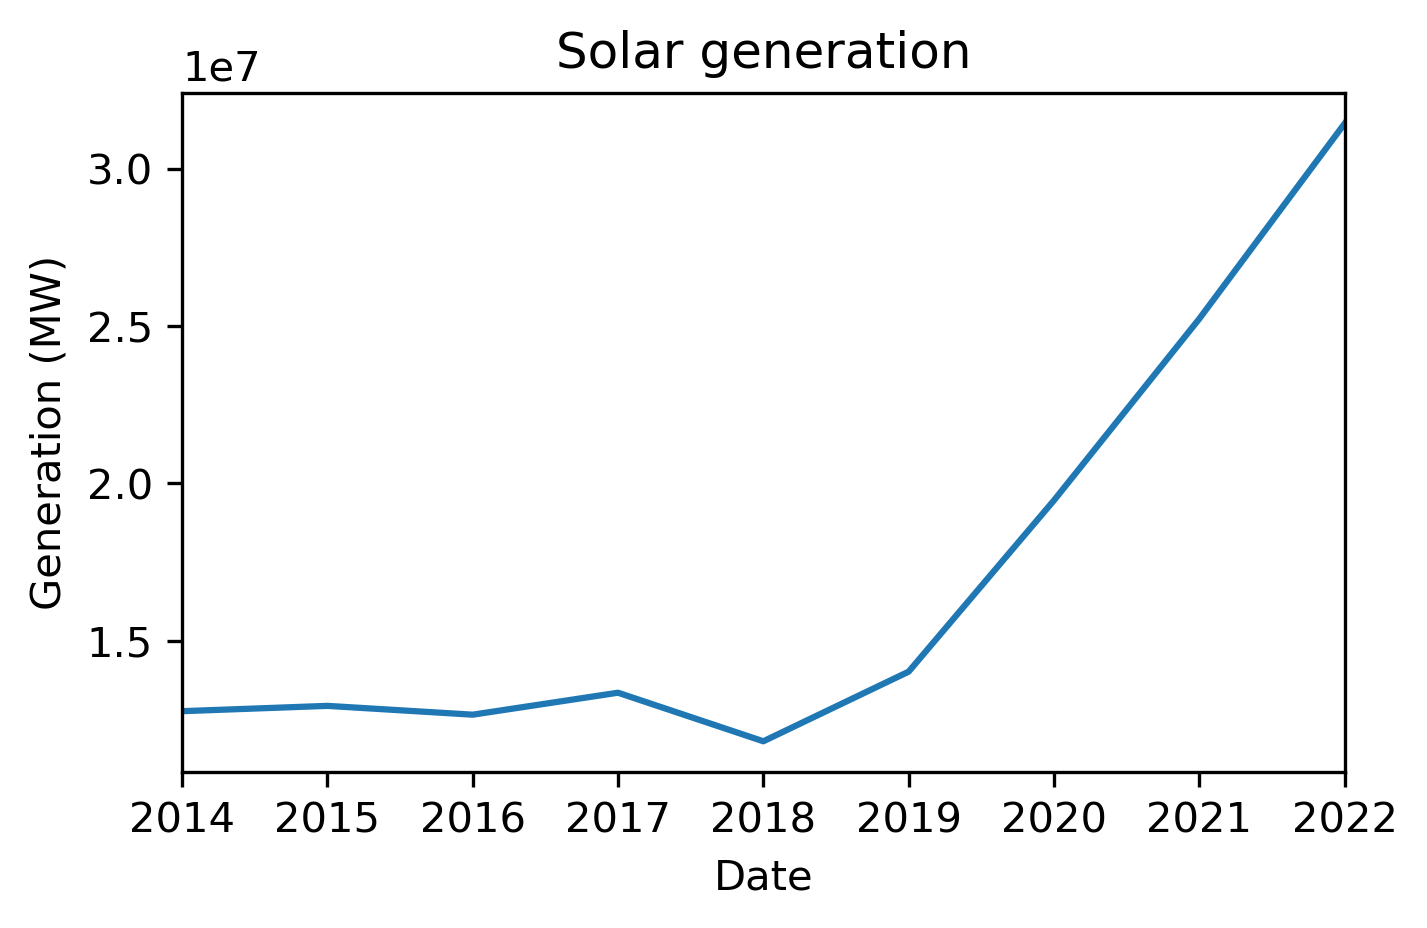
\includegraphics[width=1\linewidth]{images/analysis/solar-gen-yearly}
        \caption{Solar generation}
    \end{subfigure}

    \caption{Generation measurements aggregated by year.}
    \label{fig:gen-yearly}
\end{figure}

Observing wind power and solar generation graphs, it can be deducted that they are both technologies in expansion. In the long term, they could contribute to lower the energy price as they don't need fuel to run, just nature forces. Apart, their use will make us less dependent on other countries, making

Looking at these graphs, the author thinks that energy price could return to levels similar to before the pandemic. This year has seen a price decline, and with the help of renewable energy this price could decrease even more in the following years. Nevertheless, due to inflation, it probably won't be as low as before.